\newcommand{\institut}{Institut f\"ur Energie und  Automatisiertungstechnik}
\newcommand{\fachgebiet}{Elektronische Mess- und Diagnosetechnik}
\newcommand{\veranstaltung}{Praktikum Messdatenverarbeitung}
\newcommand{\pdfautor}{\"Ozg\"u Dogan (326 048), Timo Lausen (325 411), Boris Henckell (325 779)}
\newcommand{\autor}{\"Ozg\"u Dogan (326 048)\\ Timo Lausen (325 411)\\ Boris Henckell (325 779)}
\newcommand{\pdftitle}{Praktikum Messdatenverarbeitung  Termin 3 und 4}
\newcommand{\prototitle}{Praktikum Messdatenverarbeitung \\ Termin 3 und 4}
\newcommand{\aufgabe}{}

\newcommand{\gruppe}{Gruppe: G1 Fr 08-10}
\newcommand{\betreuer}{Betreuer: J\"urgen Funk}

\input{../../packages/tu_header_8}

% \lstlistoflistings
\definecolor{darkgray}{rgb}{0.95,0.95,0.95}
\definecolor{darkolivegreen}{HTML}{01a801}
\definecolor{functionsBlue}{HTML}{32b9b9}
\definecolor{variableRed}{rgb}{1,0,0}
\definecolor{stringBrown}{HTML}{bc8e8e} % f geht nicht

\lstset{
        %\lstset{extendedchars=true} % Umlaute an der richtigen stelle und nicht am Anfang ausgeben
        %basicstyle=\footnotesize\ttfamily,
        basicstyle=\small,
        %
        inputencoding=utf8,
        %
        tabsize=4,
        showspaces=false,
        showtabs=false,
        showstringspaces=true, % no special string spaces
        %
        backgroundcolor=\color{darkgray}, % background
        stringstyle=\color{stringBrown}\fseries, % Strings
        keywordstyle=\color{functionsBlue}\bfseries, % keywords Blau
        identifierstyle=\color{variableRed}, % variablen
        commentstyle=\color{darkolivegreen}, %  comments
        %
        breaklines=true,
        %
        numbers=left,
        numberstyle=\tiny,
        stepnumber=1,
        numbersep=7pt,
        %
        frame=single,
        columns=flexible,
        %
        xleftmargin=-2cm,
        xrightmargin=-1.5cm,
        %
        language=Matlab
}


%---------------------------------------------------------------------
%---------------------------------------------------------------------
%---------------------------------------------------------------------

\section{Vorbereitungsaufgaben}
\begin{quote}
    \subsection{Vorbereitungsaufgaben Termin 3}
    \begin{quote}
        \subsubsection{Sinusfunktion erzeugen und DFT erstellen}
        \begin{quote}
            Die erste Vorbereitungsaufgabe hatte das Ziel einen verschobenes Sinussignal zu erzeugen, die DFT davon zu
            betimmen und dieses zu plotten. Der dazugehärige Quelltext sinus2.m befindet sich im Anhang.
            \begin{figure}[H]
            \centering
                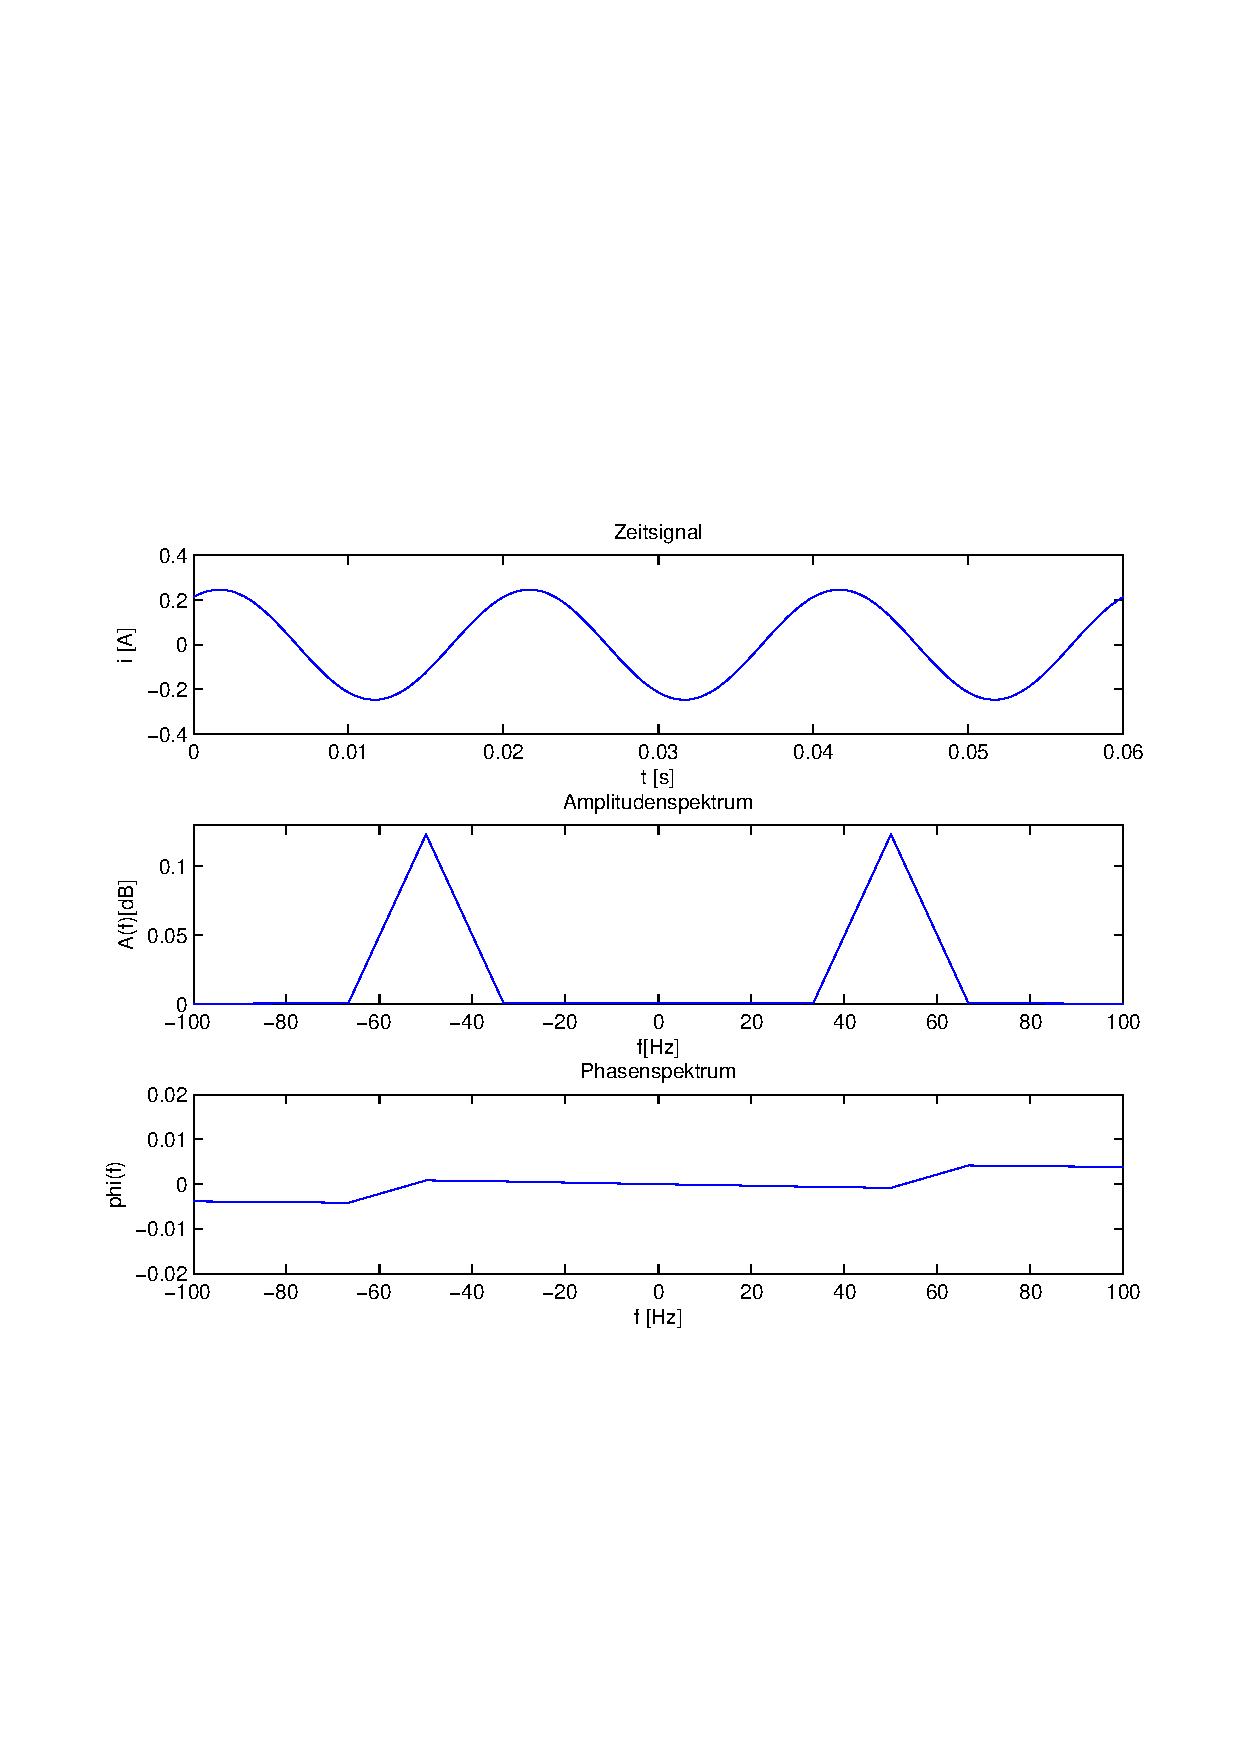
\includegraphics[scale=0.5, trim = 0cm 0cm 0cm 0cm, clip]{./Bilder/VerschobenerSinusAufgabe1}
                    \caption{Verschobener Sinus}
                    \label{fig:./Bilder/VerschobenerSinusAufgabe1}
            \end{figure}
        
        \end{quote}
        
    	\subsubsection{Angeschnittene Sinusfunktion}
        \begin{quote}
            In der zweiten Vorbereitungsaufgabe sollte eine Matlab-Funktion geschrieben werden die einen angeschnittene
            Sinusfunktion simuliuliert.\\
            Um diese Funktion zu erstellen haben wir eine for Schleife imlementiert, die den gesamten zeitvektor t
            durchläuft. Für jeden Durchlauf wird getestet, wo sich der jeweilige Zeitpunkt im Verhältniss zum halben
            sinussignal befindet. Anschließend wird in der if abfrage bestimmt, ob sich dieser Zeitpunkt relativ zur halben
            Periode des Sinussignals vor oder hinter dem Phasenanschnittswinkel befindet. Abhängig davon wird der
            dentsprechenden Stelle im Ausgabevektor der Wert $0$ oder der Wert den die Sinusfunktion ermittelt, übergeben.\\
            Wir haben die Graphen für folgende Phasenanschnittswinkel $ \alpha = 0, \frac{1}{8} \pi, \frac{1}{4}
            \pi, \frac{3}{8} \pi, \frac{1}{2} \pi,\frac{5}{8} \pi, \frac{3}{4} \pi, \frac{7}{8} \pi$ und $\pi$
            geplottet.\\
            Der dazugehärige Quelltext befindet sich im Anhang.
        \end{quote}
        
        \subsubsection{Effektivwert des Stroms im Zeitbereich}
        \begin{quote}
            Für den Effektivwert des Stroms im Zeitbereich ermitteln wir die Wurzel des Mittelwertes des Quadrats des
            Stromvektors.\\
            Der dazugehörige Quelltext befindet sich im Anhang.
        \end{quote}
        
        \subsubsection{Effektivwert des Stroms im Frequenzbereich}
        \begin{quote}
            Den Effektivwert des Stroms im Frequenzbereich ermitteln wir ähnlich wie den Effektivwert des Stroms im
            Zeitbereich. Das Parsevalschen-Theorem besagt, dass die Energien eines Signals im Zeitbereich gleich seiner
            Energie im Frequenzbereich ist.\cite{PasevalscheTheorem}\\
            \begin{equation*}
            	\begin{split}
            		\sum_{n=0}^{N-1} |x[n]|^2 = \frac{1}{N} \sum_{k=0}^{N-1} |X[k]|^2
            	\end{split}
            \end{equation*}
            
            Der dazugehörige Quelltext befindet sich im Anhang.
            \end{quote}
        \subsubsection{Ergebnisse Vorbereitungsaufgaben}
        \begin{quote}
                                    %4 Grafiken:
                \begin{center}
                \begin{tabular}{ll}
    
                \hspace{-11em}
                    \begin{minipage}{0.6\textwidth}
    
                        \begin{figure}[H]
                            \label{fig:}
                            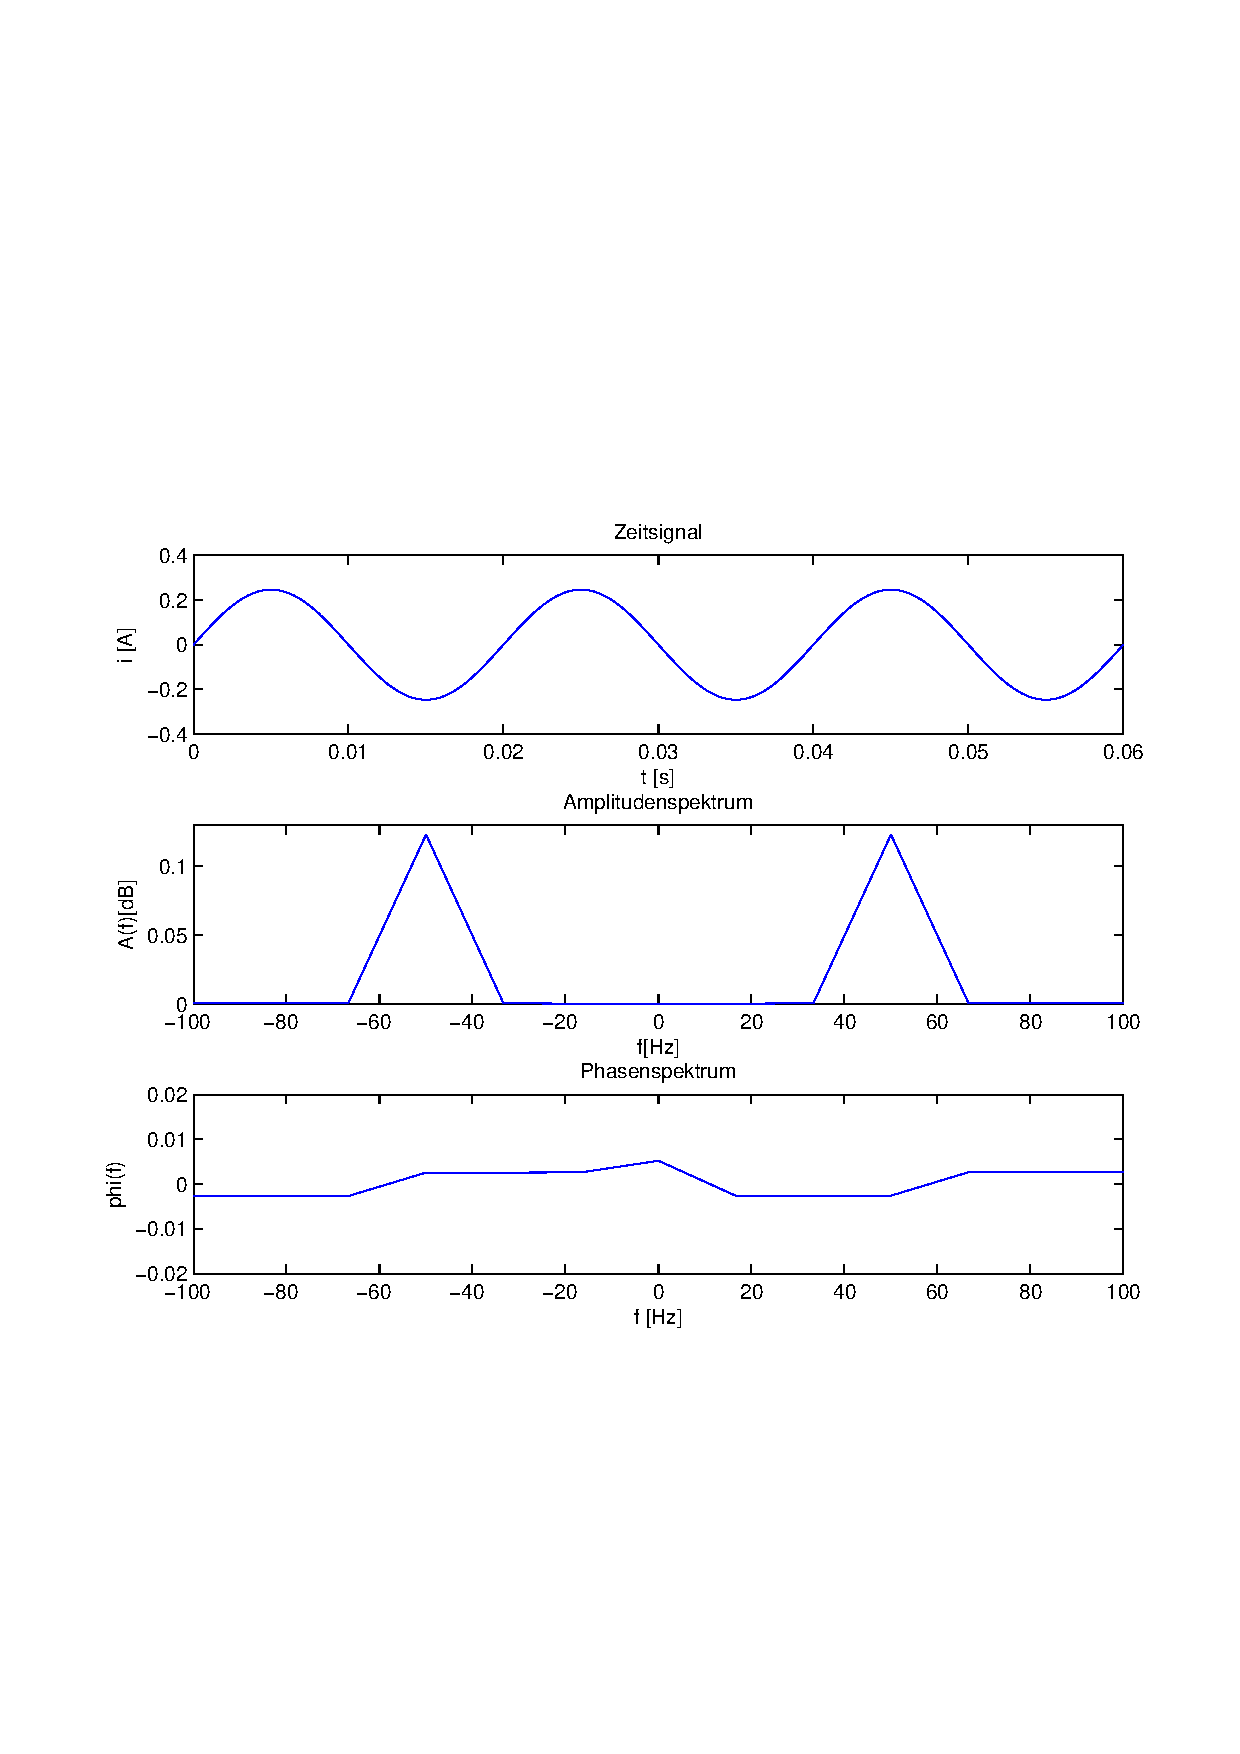
\includegraphics[scale=0.5, trim = 2cm 7cm 1.5cm 8.5cm, clip]{./Bilder/Phasenanschnitt08pi.pdf}
                            %FIXME [width=640px,
                             %height=474px]
                            \caption{Sinussignal mit Phasenanschnitt von $0$}
                        \end{figure}
    
                    \end{minipage}
                    \begin{minipage}{0.6\textwidth}
    
                        \begin{figure}[H]
                            \label{fig:}
                            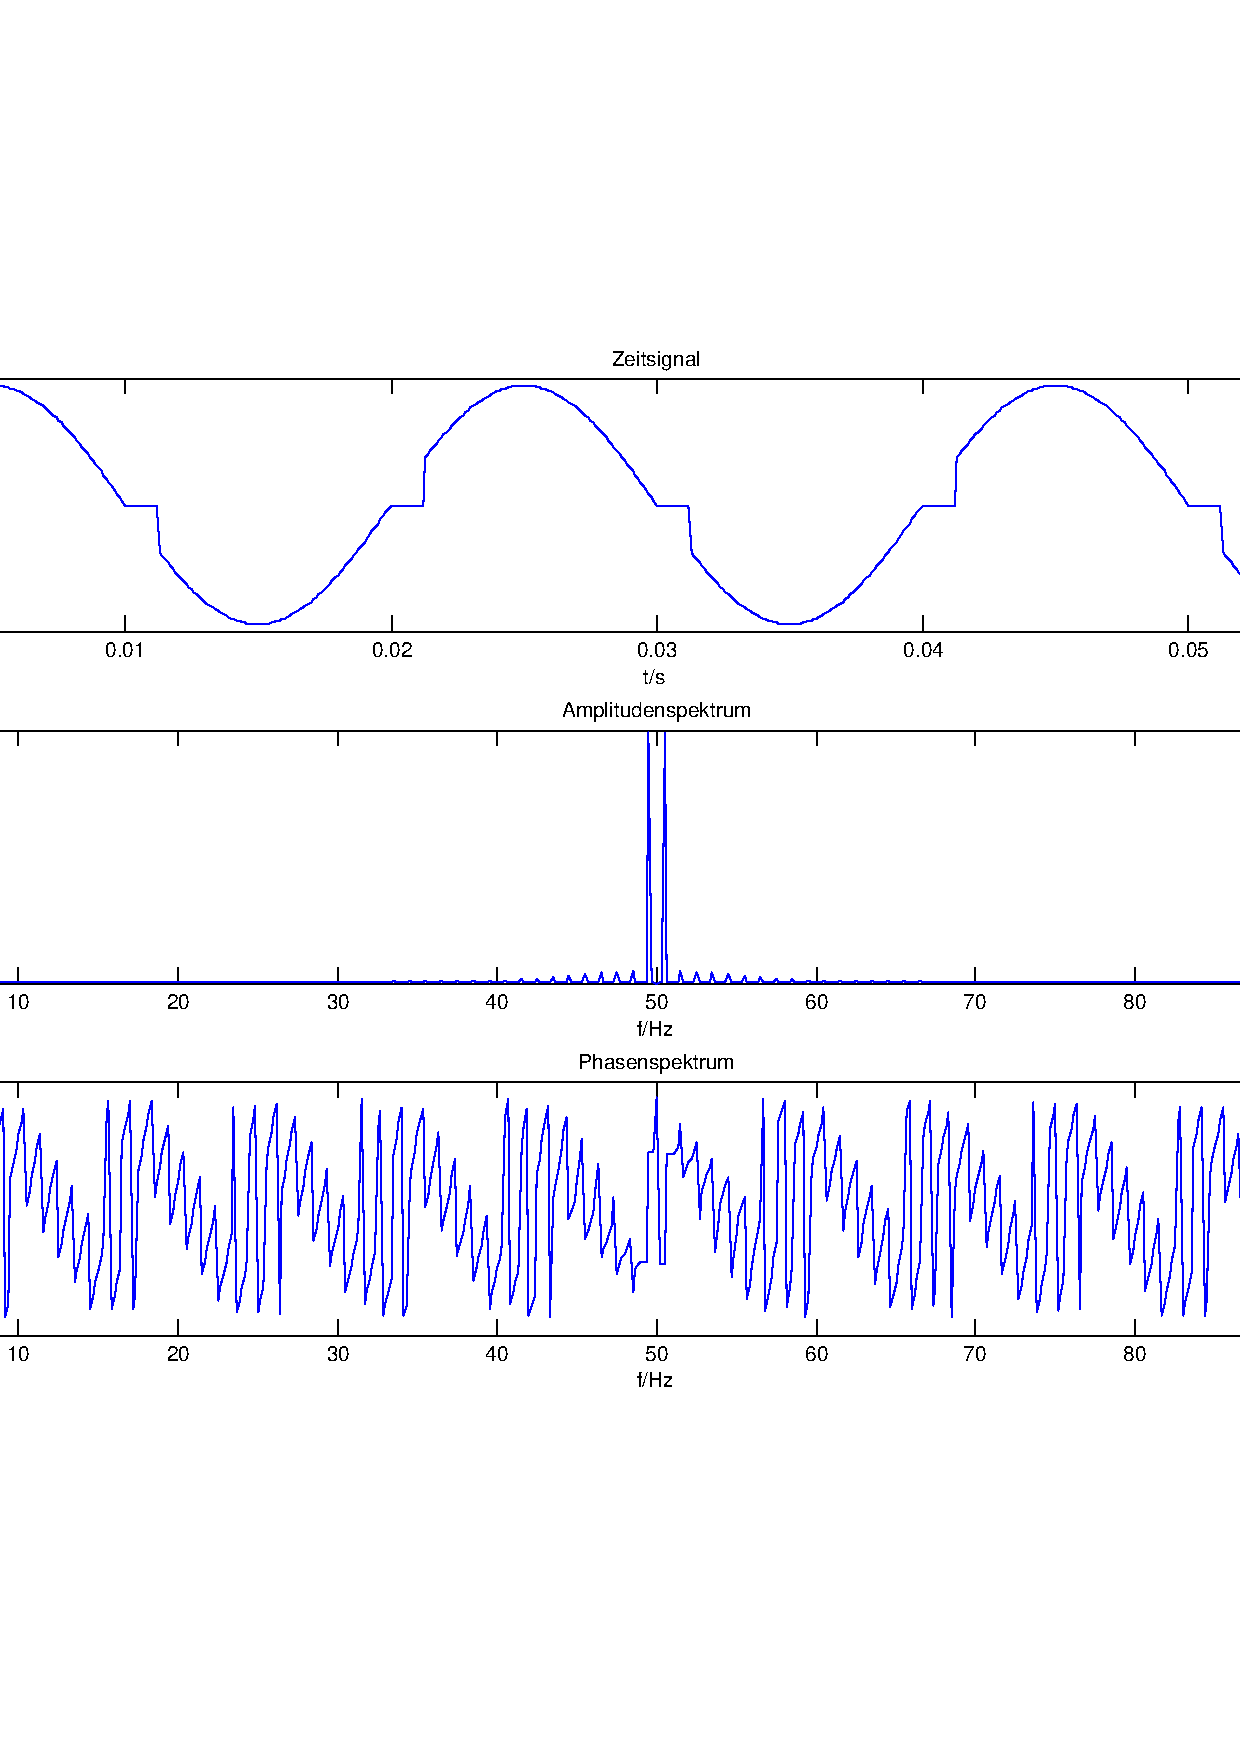
\includegraphics[scale=0.5, trim = 2cm 7cm 1.5cm 8.5cm, clip]{./Bilder/Phasenanschnitt18pi.pdf}
                            %FIXME [width=640px,
                             %height=474px]
                            \caption{Sinussignal mit Phasenanschnitt von $\frac{1}{8}/pi$}
                        \end{figure}
                    \vspace{-1.5em}
    
                    \end{minipage}
    
                \end{tabular}
                \end{center}
    
                            %4 Grafiken:
                \begin{center}
                \begin{tabular}{ll}
    
                \hspace{-11em}
                    \begin{minipage}{0.6\textwidth}
    
                        \begin{figure}[H]
                            \label{fig:}
                            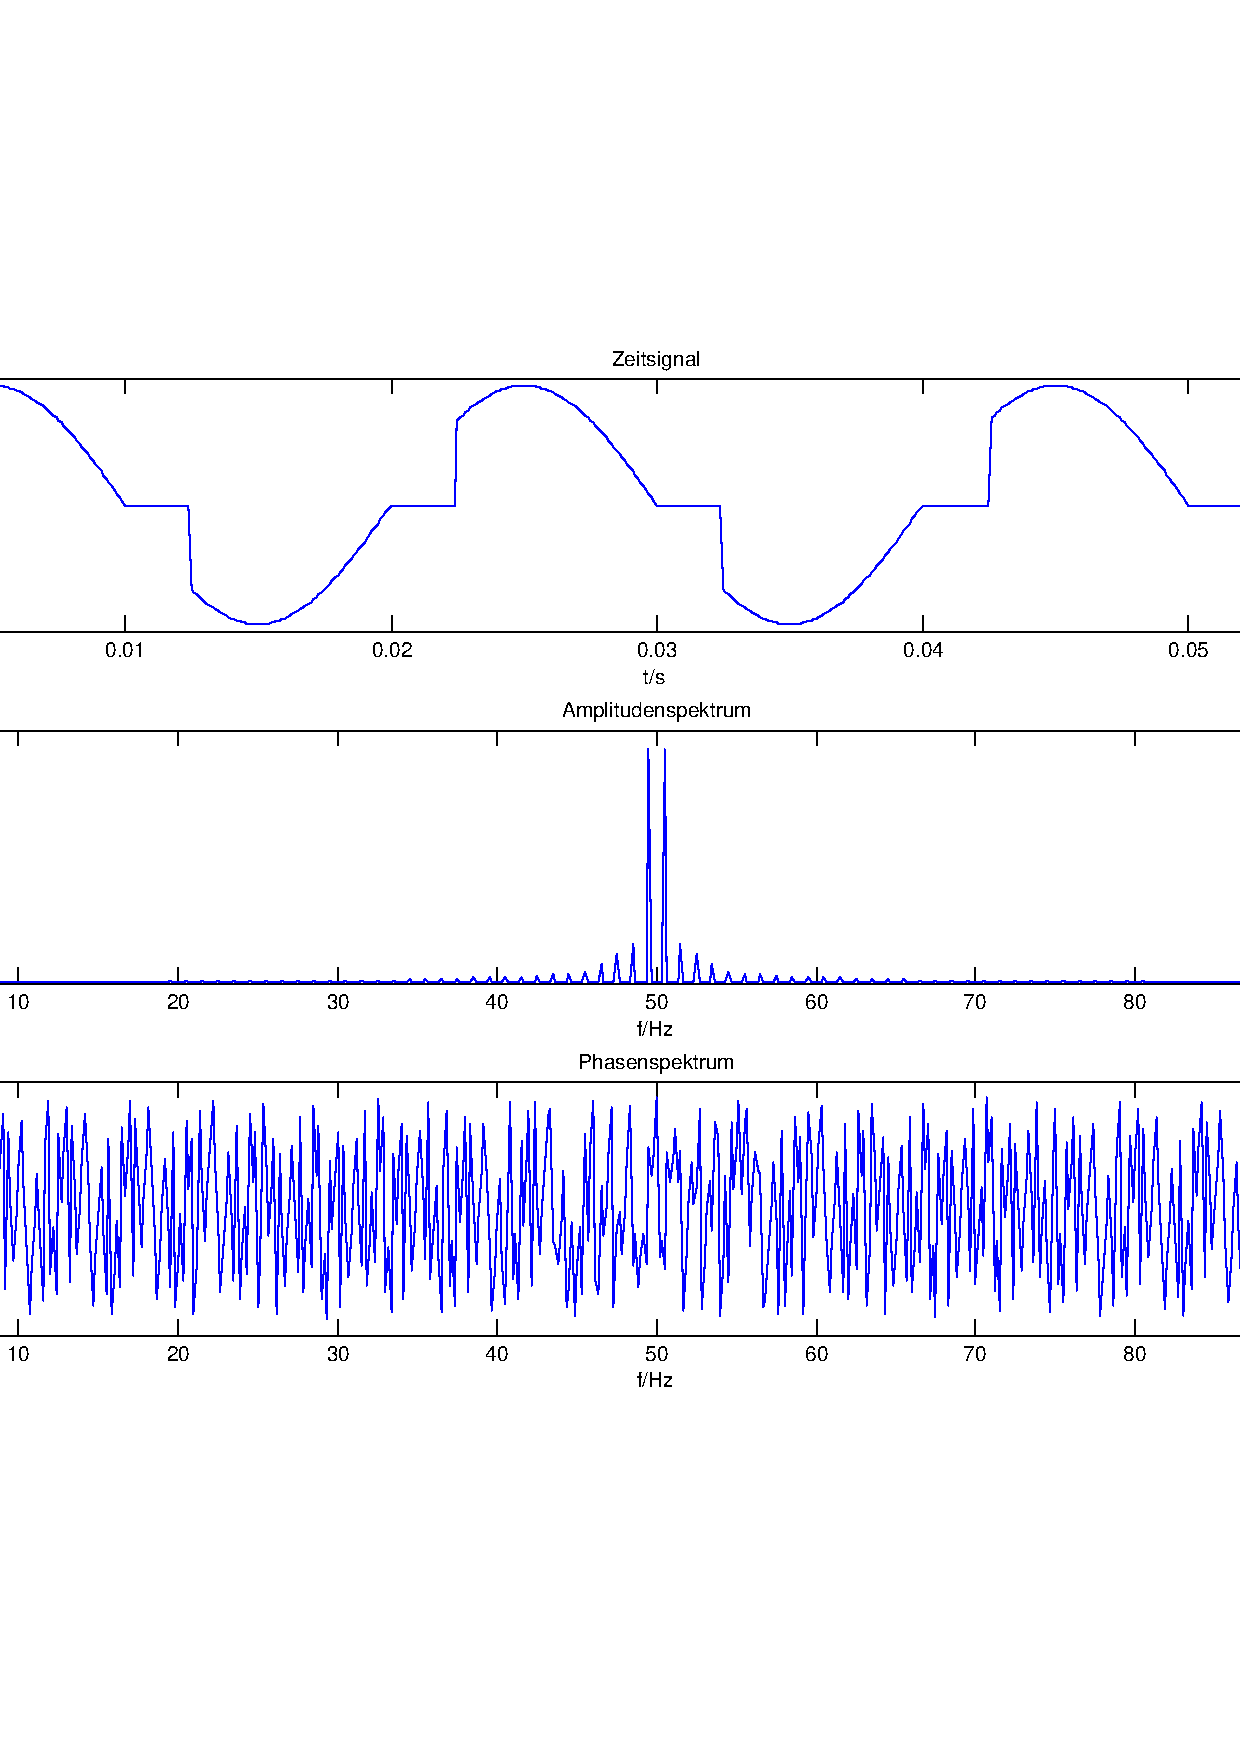
\includegraphics[scale=0.5, trim = 2cm 7cm 1.5cm 8.5cm, clip]{./Bilder/Phasenanschnitt28pi.pdf} %FIXME [width=640px,
                            % height=474px]
                            \caption{Sinussignal mit Phasenanschnitt von $\frac{1}{4}/pi$}
                        \end{figure}
    
                    \end{minipage}
                    \begin{minipage}{0.6\textwidth}
    
                         \begin{figure}[H]
                            \label{fig:}
                            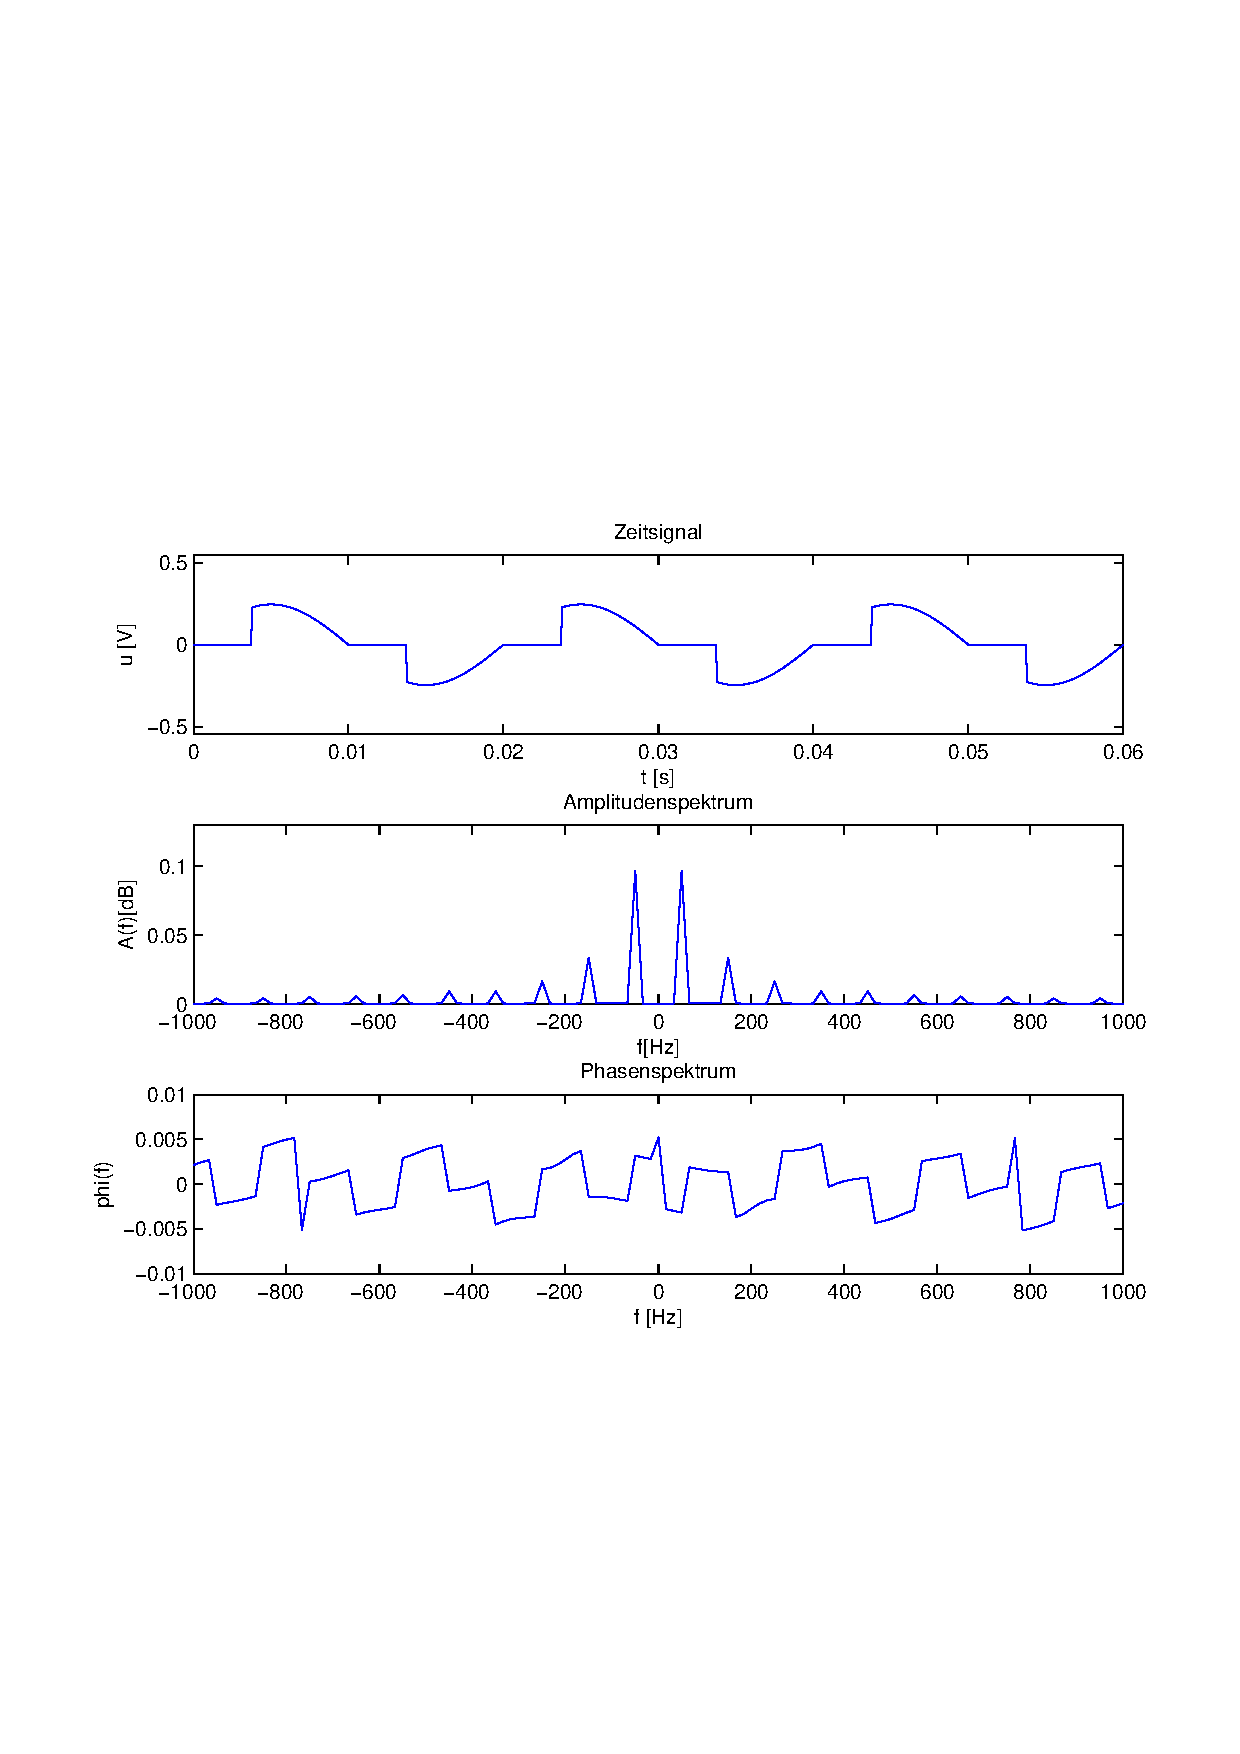
\includegraphics[scale=0.5, trim = 2cm 7cm 1.5cm 8.5cm, clip]{./Bilder/Phasenanschnitt38pi.pdf} %FIXME [width=640px,
                            % height=474px]
                            \caption{Sinussignal mit Phasenanschnitt von $\frac{3}{8}/pi$}
                        \end{figure}
                   \vspace{-1.5em}
    
                    \end{minipage}
    
                \end{tabular}
                \end{center}
    
                            %4 Grafiken:
                \begin{center}
                \begin{tabular}{ll}
    
                \hspace{-11em}
                    \begin{minipage}{0.6\textwidth}
    
                        \begin{figure}[H]
                            \label{fig:}
                            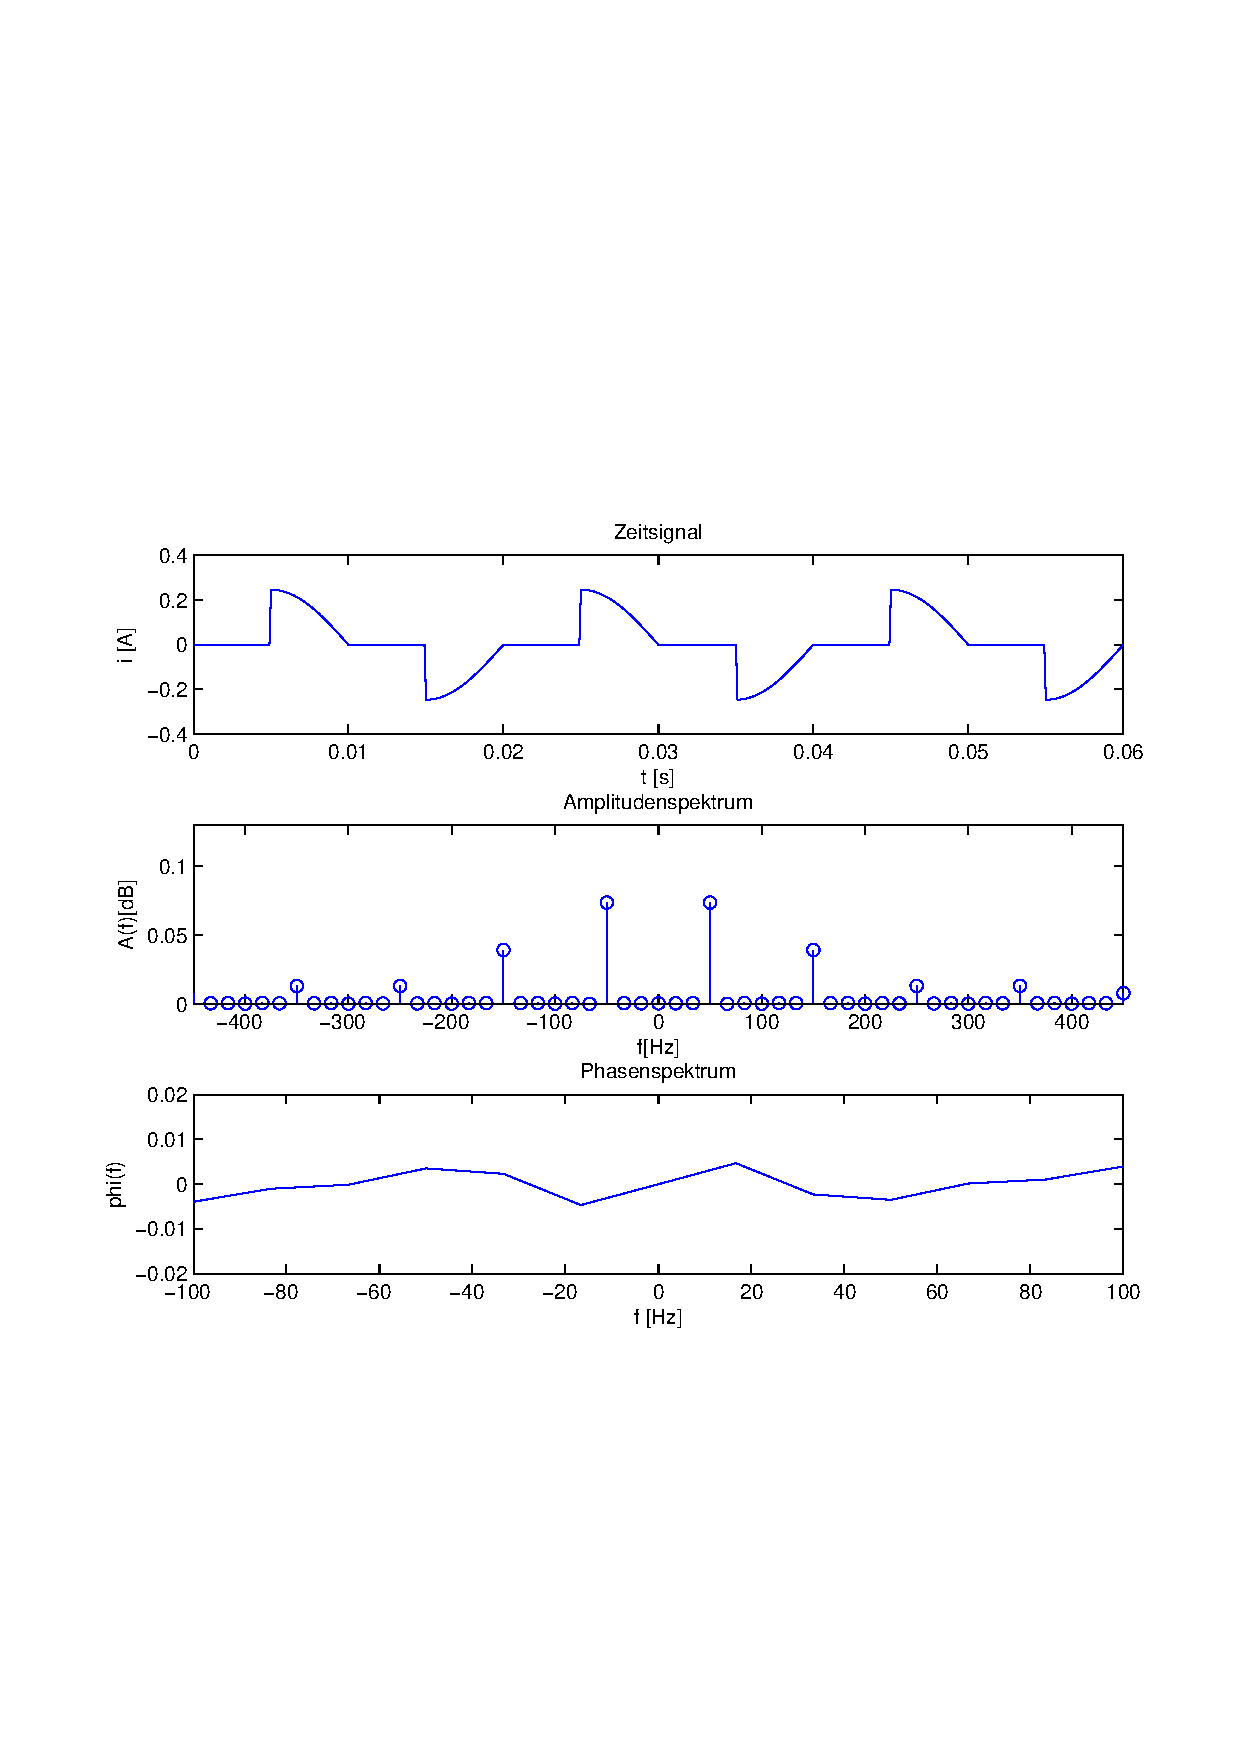
\includegraphics[scale=0.5, trim = 2cm 7cm 1.5cm 8.5cm, clip]{./Bilder/Phasenanschnitt48pi.pdf} %FIXME [width=640px,
                            % height=474px]
                            \caption{Sinussignal mit Phasenanschnitt von $\frac{1}{2}/pi$}
                        \end{figure}
    
                    \end{minipage}
                    \begin{minipage}{0.6\textwidth}
    
                       \begin{figure}[H]
                            \label{fig:}
                            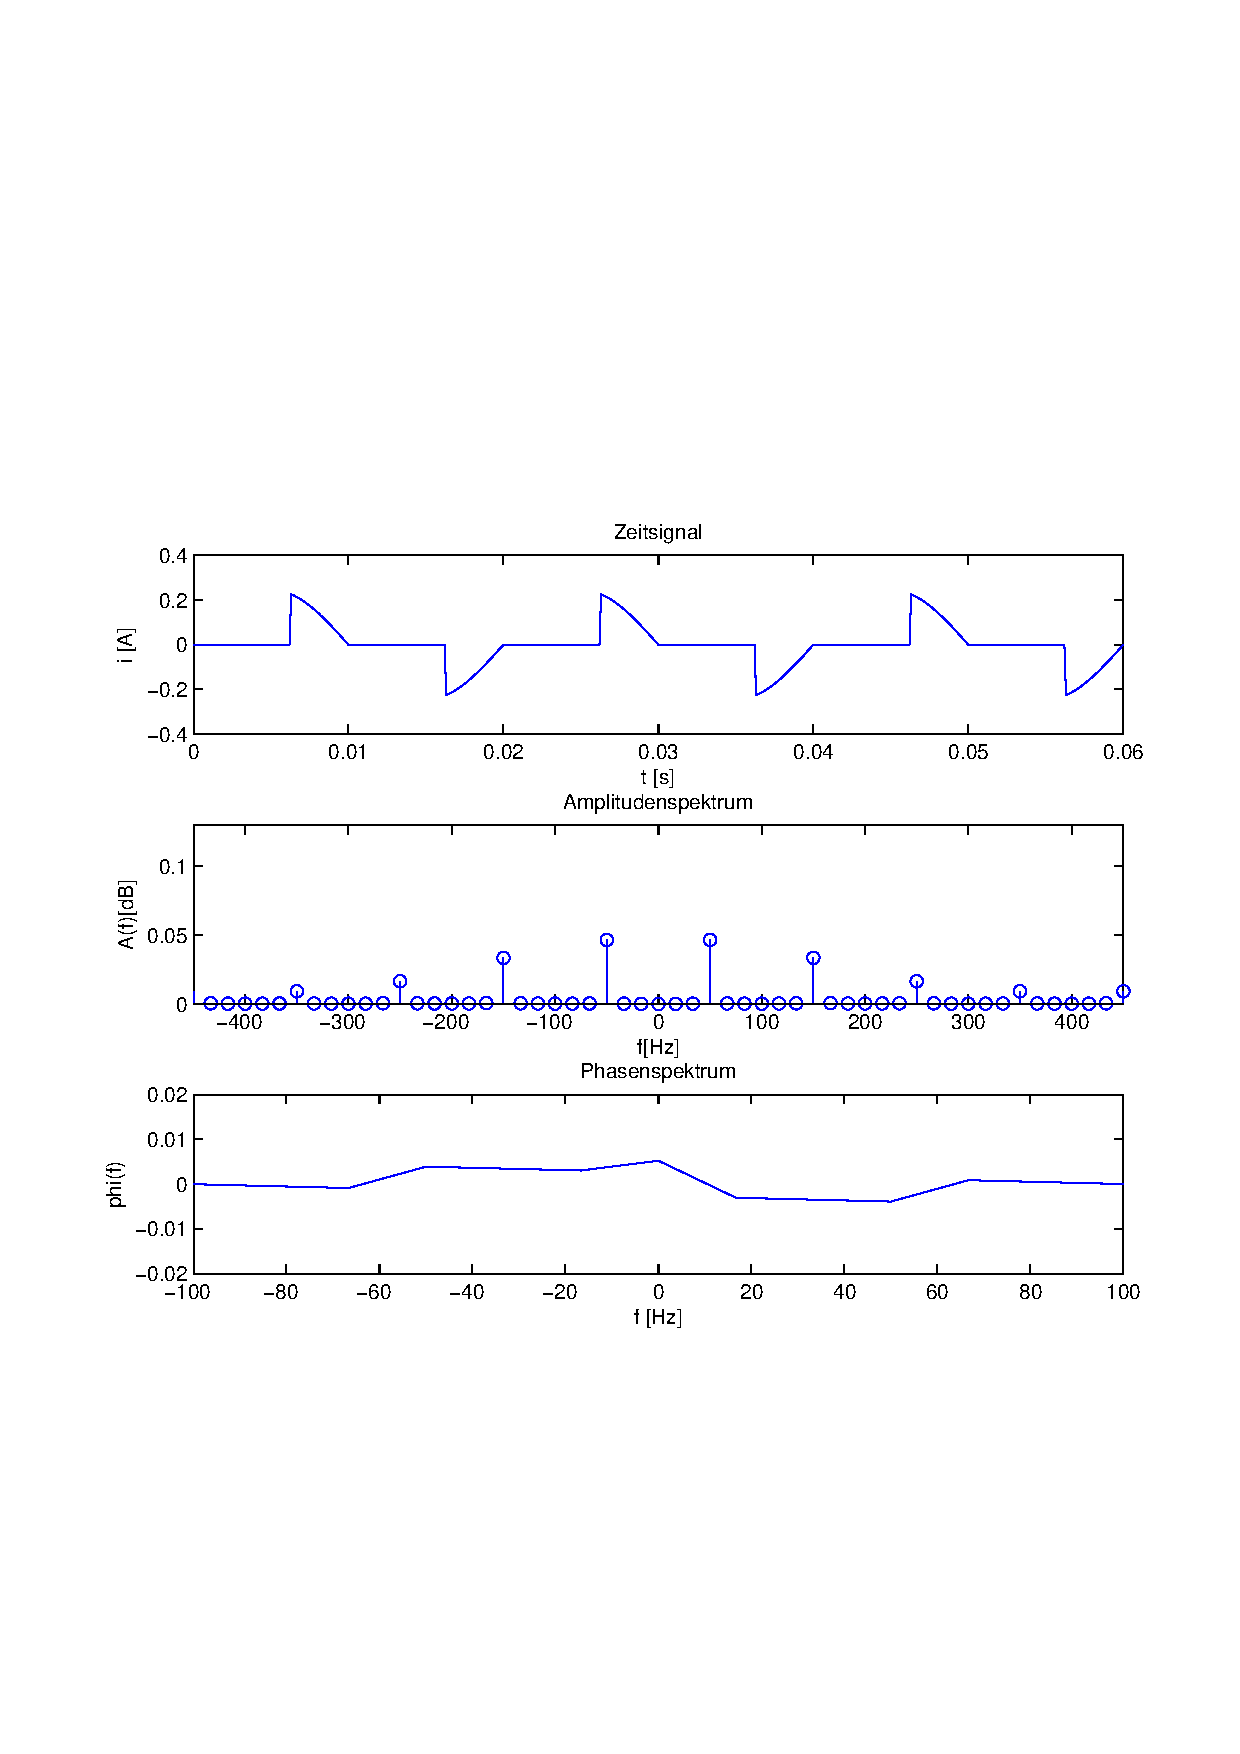
\includegraphics[scale=0.5, trim = 2cm 7cm 1.5cm 8.5cm, clip]{./Bilder/Phasenanschnitt58pi.pdf} %FIXME [width=640px,
                            % height=474px]
                            \caption{Sinussignal mit Phasenanschnitt von $\frac{5}{8}/pi$}
                        \end{figure}
                     \vspace{-1.5em}
    
                    \end{minipage}
    
                \end{tabular}
                \end{center}
    
                   %4 Grafiken:
                \begin{center}
                \begin{tabular}{ll}
    
                \hspace{-11em}
                    \begin{minipage}{0.6\textwidth}
    
                        \begin{figure}[H]
                            \label{fig:}
                            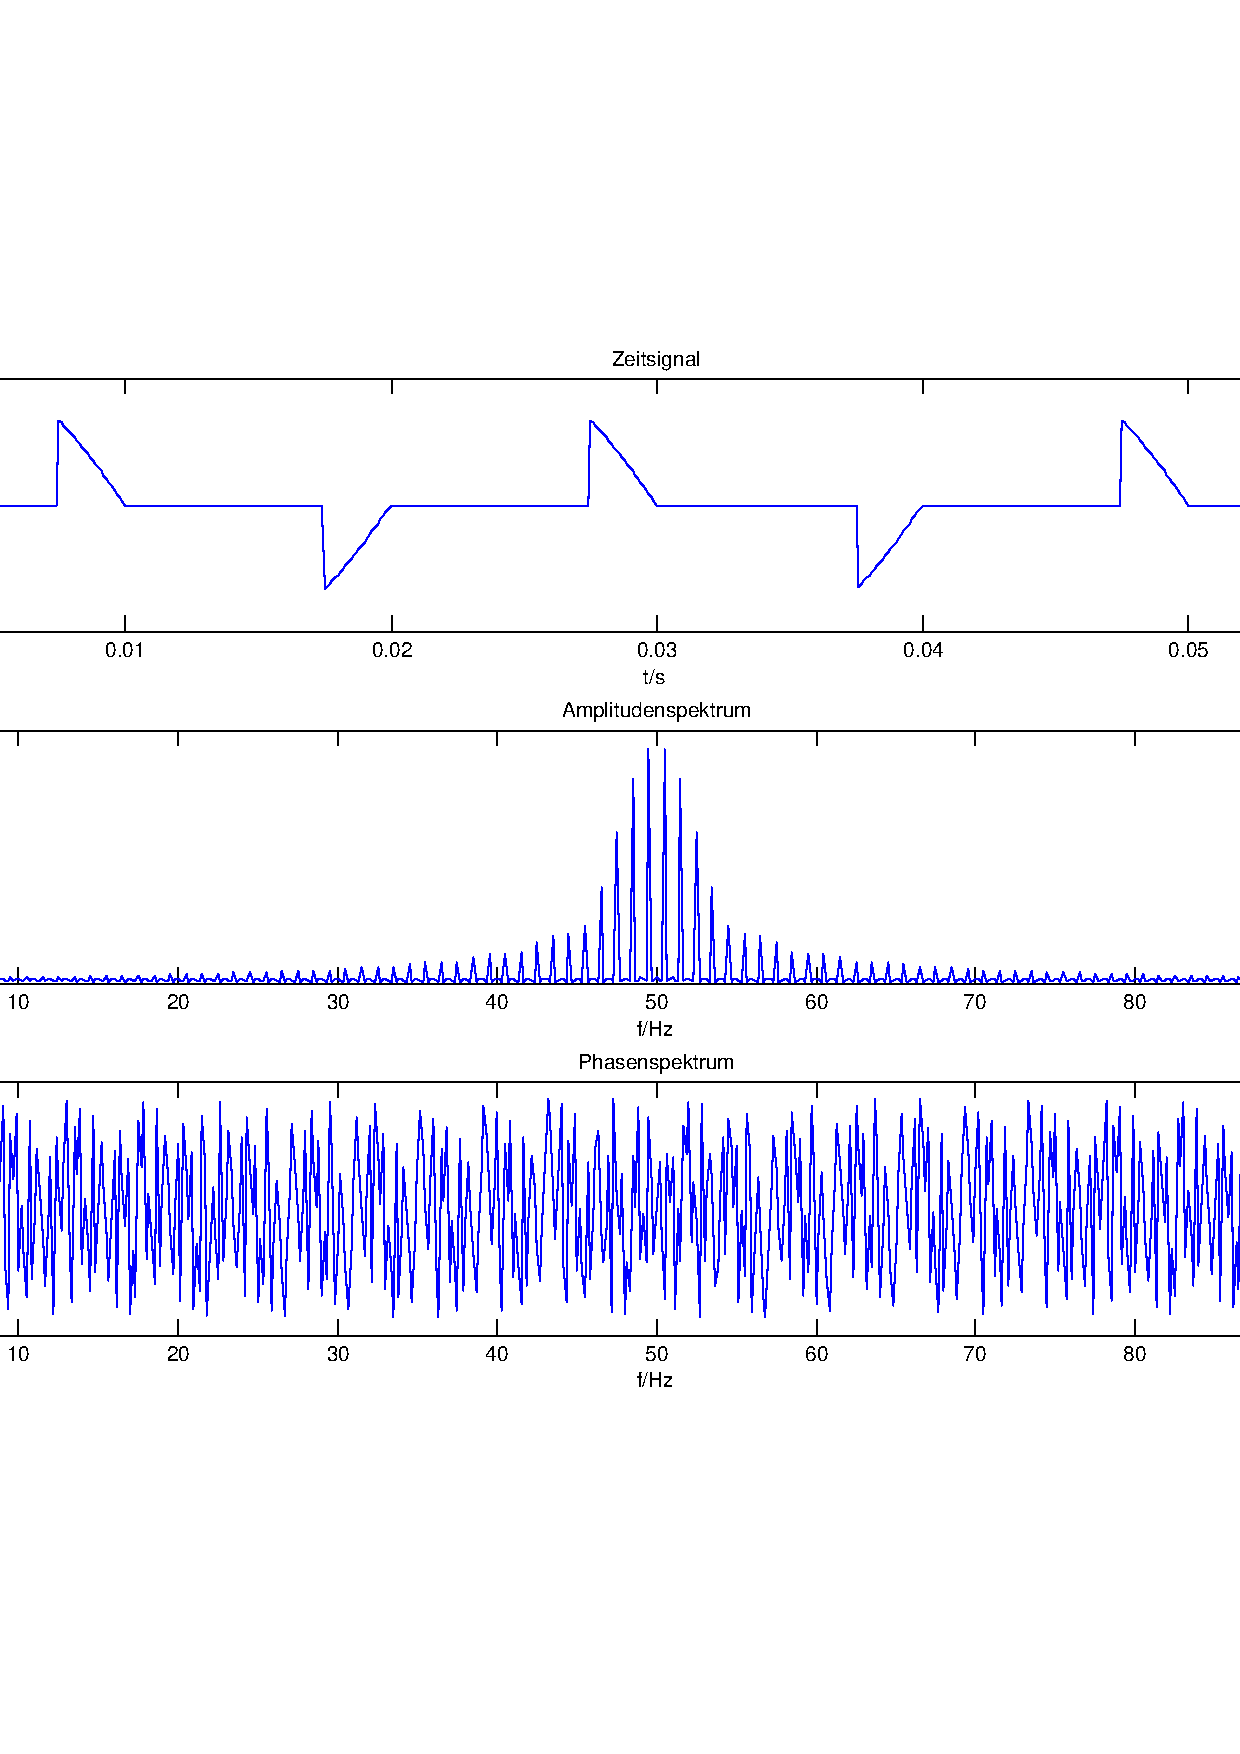
\includegraphics[scale=0.5, trim = 2cm 7cm 1.5cm 8.5cm, clip]{./Bilder/Phasenanschnitt68pi.pdf} %FIXME [width=640px,
                            % height=474px]
                            \caption{Sinussignal mit Phasenanschnitt von $\frac{3}{4}/pi$}
                        \end{figure}
    
                    \end{minipage}
                    \begin{minipage}{0.6\textwidth}
    
                       \begin{figure}[H]
                            \label{fig:}
                            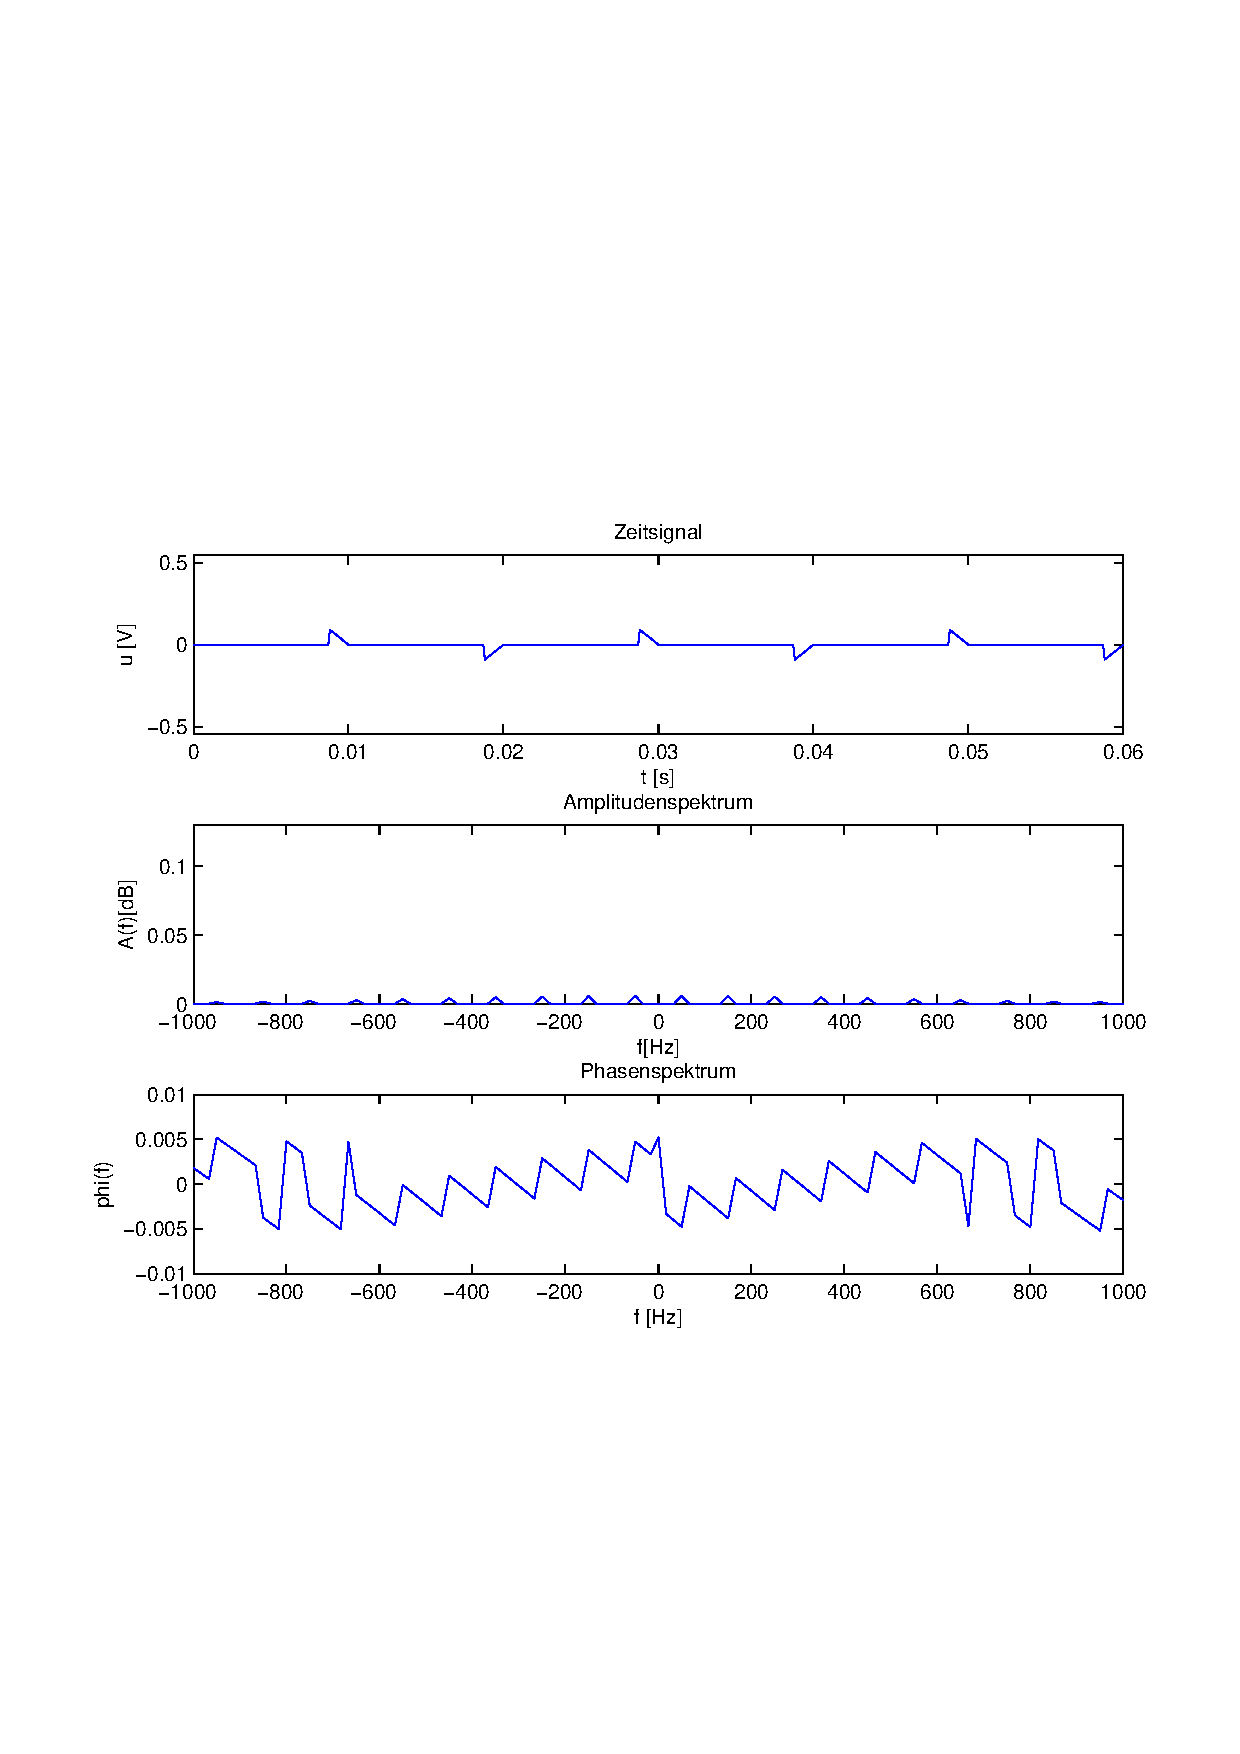
\includegraphics[scale=0.5, trim = 2cm 7cm 1.5cm 8.5cm, clip]{./Bilder/Phasenanschnitt78pi.pdf} %FIXME [width=640px,
                            % height=474px]
                            \caption{Sinussignal mit Phasenanschnitt von $\frac{7}{8}/pi$}
                        \end{figure}
                     \vspace{-1.5em}
    
                    \end{minipage}
    
                \end{tabular}
                \end{center}
                
                   %4 Grafiken:
                \begin{center}
                \begin{tabular}{ll}
    
                \hspace{-4em}
                    \begin{minipage}{0.6\textwidth}
    
                        \begin{figure}[H]
                            \label{fig:}
                            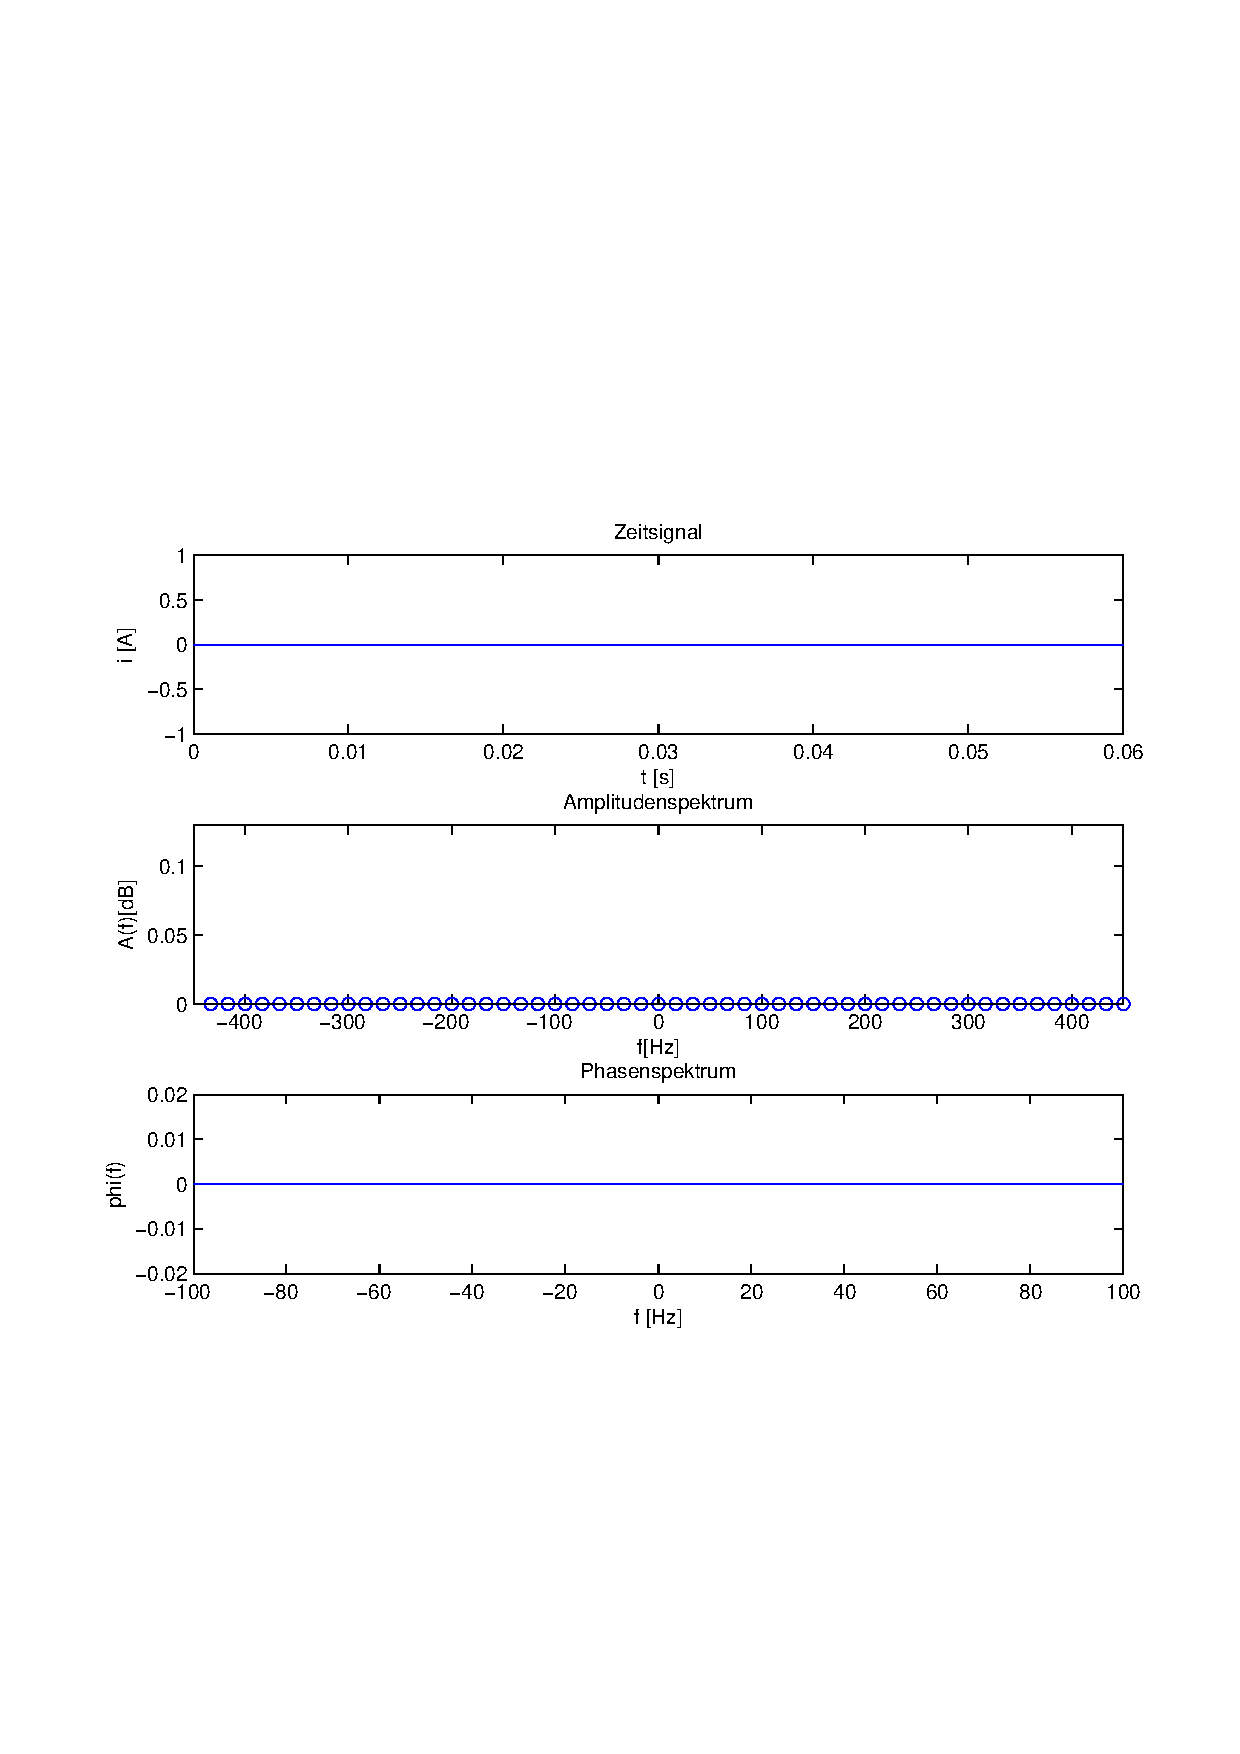
\includegraphics[scale=0.5, trim = 2cm 7cm 1.5cm 8.5cm, clip]{./Bilder/Phasenanschnitt88pi.pdf} %FIXME [width=640px,
                            % height=474px]
                            \caption{Sinussignal mit Phasenanschnitt von $/pi$}
                        \end{figure}
    
                    \end{minipage}
    
                \end{tabular}
                \end{center}
                 \begin{center}
                     \begin{tabular}{|c|c|c|}
                                 
                       \hline
                       $\alpha $ & $i_{eff}$ (Zeitbereich) & $i_{eff}$ Frequenzbereich\\ \hline
                       $0$ & 3,5326 & 3,5326 \\ \hline
                       $\frac{1}{8} \pi$ & 3,5105 & 3,5105 \\ \hline
                       $\frac{1}{4} \pi$ & 3,3744 & 3,3744 \\ \hline
                       $\frac{3}{8} \pi$ & 3,0338 & 3,0338 \\ \hline
                       $\frac{1}{2} \pi$ & 2,5145 & 2,5145 \\ \hline
                       $\frac{5}{8} \pi$ & 1,8097 & 1,8097 \\ \hline
                       $\frac{3}{4} \pi$ & 1,0748 & 1,0748 \\ \hline
                       $\frac{7}{8} \pi$ & 0,3940 & 0,3940 \\ \hline
                       $ \pi$ & 0 & 0 \\ \hline
                             
               
                     \end{tabular}
                 \end{center}        
        \end{quote}
    \end{quote}
    \subsection{Vorbereitungsaufgaben Termin 4}
    \begin{quote}
        In dem zweiten Teil der Vorbereitungsaufgaben ging es um Fensterung. Mit
        unterschiedlichen Fensterfunktionen kann man Analysefenster erschaffen,
        die ein ganzzahliges Vielfaches der Periodendauer des Messsignals lang
        sind. Somit kann man bei der Untersuchung der Signale Leck-Effekte
        verhindern.\\
       
        \subsubsection{Matlabfunktion-Spektrum}
		\begin{quote}
            Dafür machten wir uns mit unterschiedlichen Fensterfunktionen vertraut und schrieben eine MATLAB Funktion,
            mit der ein Fenster generiert werden konnte, dessen Länge genau einer Periodenlänge des verwendeten Signals
            entspricht. Zusätzlich wurden Fenster und Signal überlagert und die DFT gebildet, Betrags- und
            Phasenspektren wurden geplottet.\\
            Das dazugehärige Matlabscripte Spektrum.m sowie Vorbereitungsaufgabe42.m befindet sich im Anhang.\\
            In diesem Skript haben wir ein Sinussignal mit der Frequenz $100$Hz erzeugt und jeweils mit einem Rechteck-,
            einem BlackMan-, einem Hanning- sowie einem verkürztem Hanningfenster multipliziert.\\
            Die Plotts dazu sind hier:
            
            \begin{figure}[H]
            \centering
                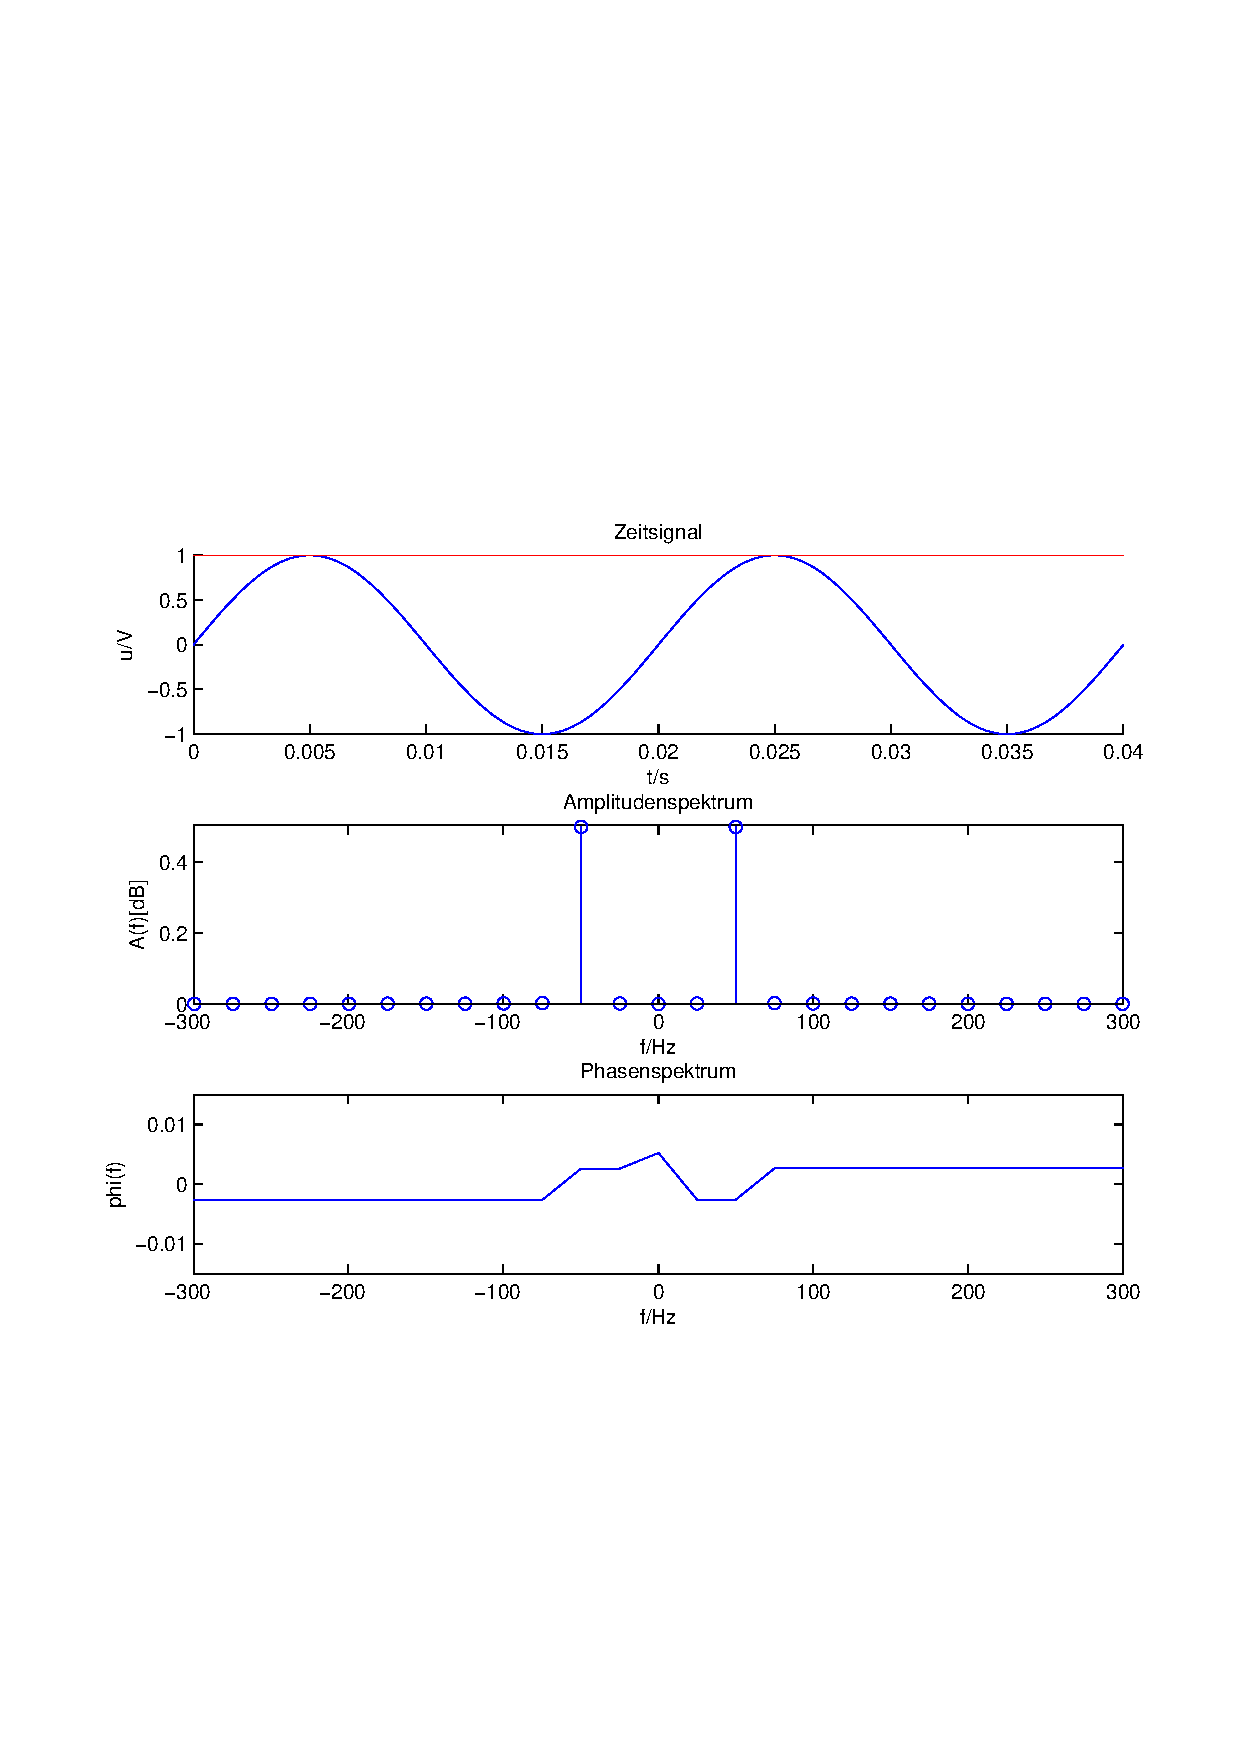
\includegraphics[scale=0.5, trim = 1.5cm 7cm 1.5cm 8cm, clip]{./Bilder/Rechteckwindow}
                    \caption{Rechteckwindow}
            \end{figure}
            
            \begin{figure}[H]
            \centering
                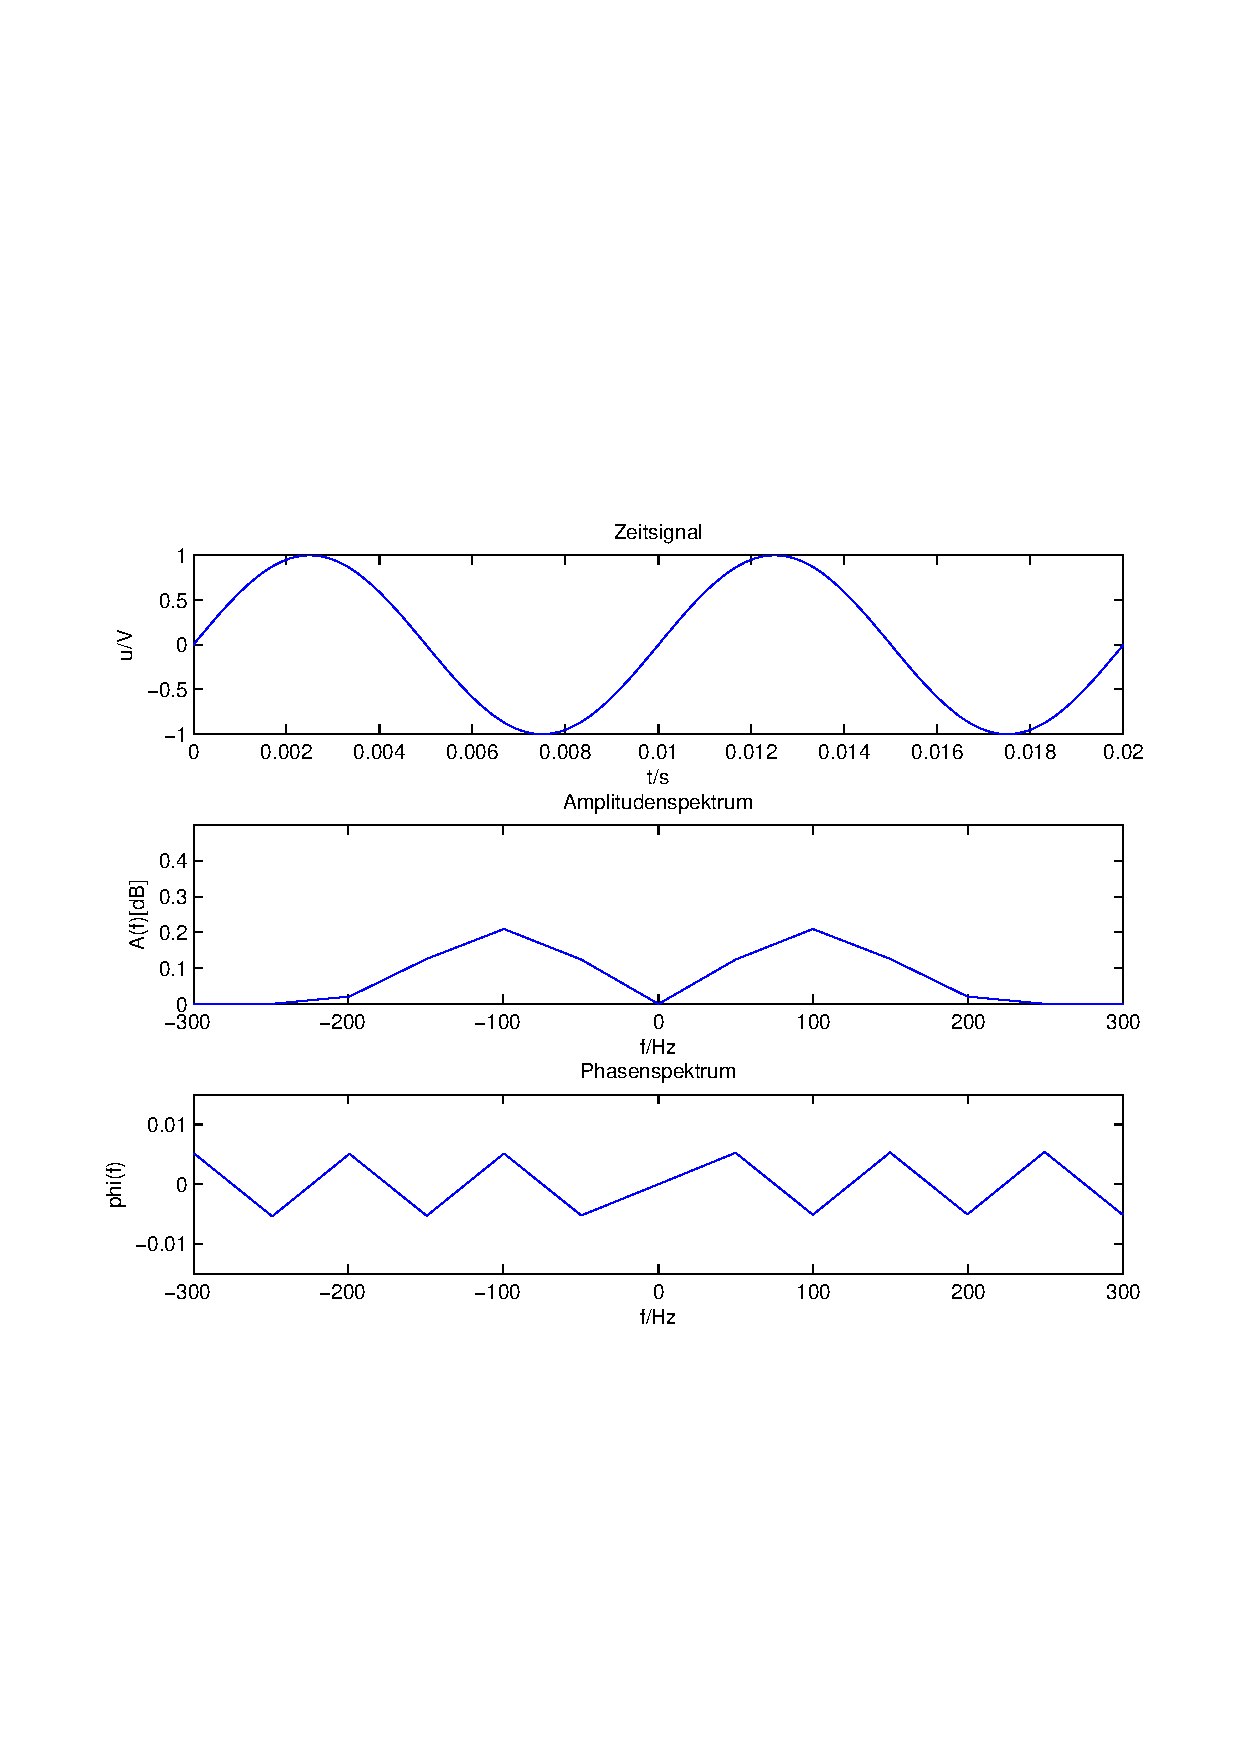
\includegraphics[scale=0.5, trim = 1.5cm 7cm 1.5cm 8cm, clip]{./Bilder/BlackManwindow}
                    \caption{BlackManwindow}
            \end{figure}
    
            \begin{figure}[H]
            \centering
                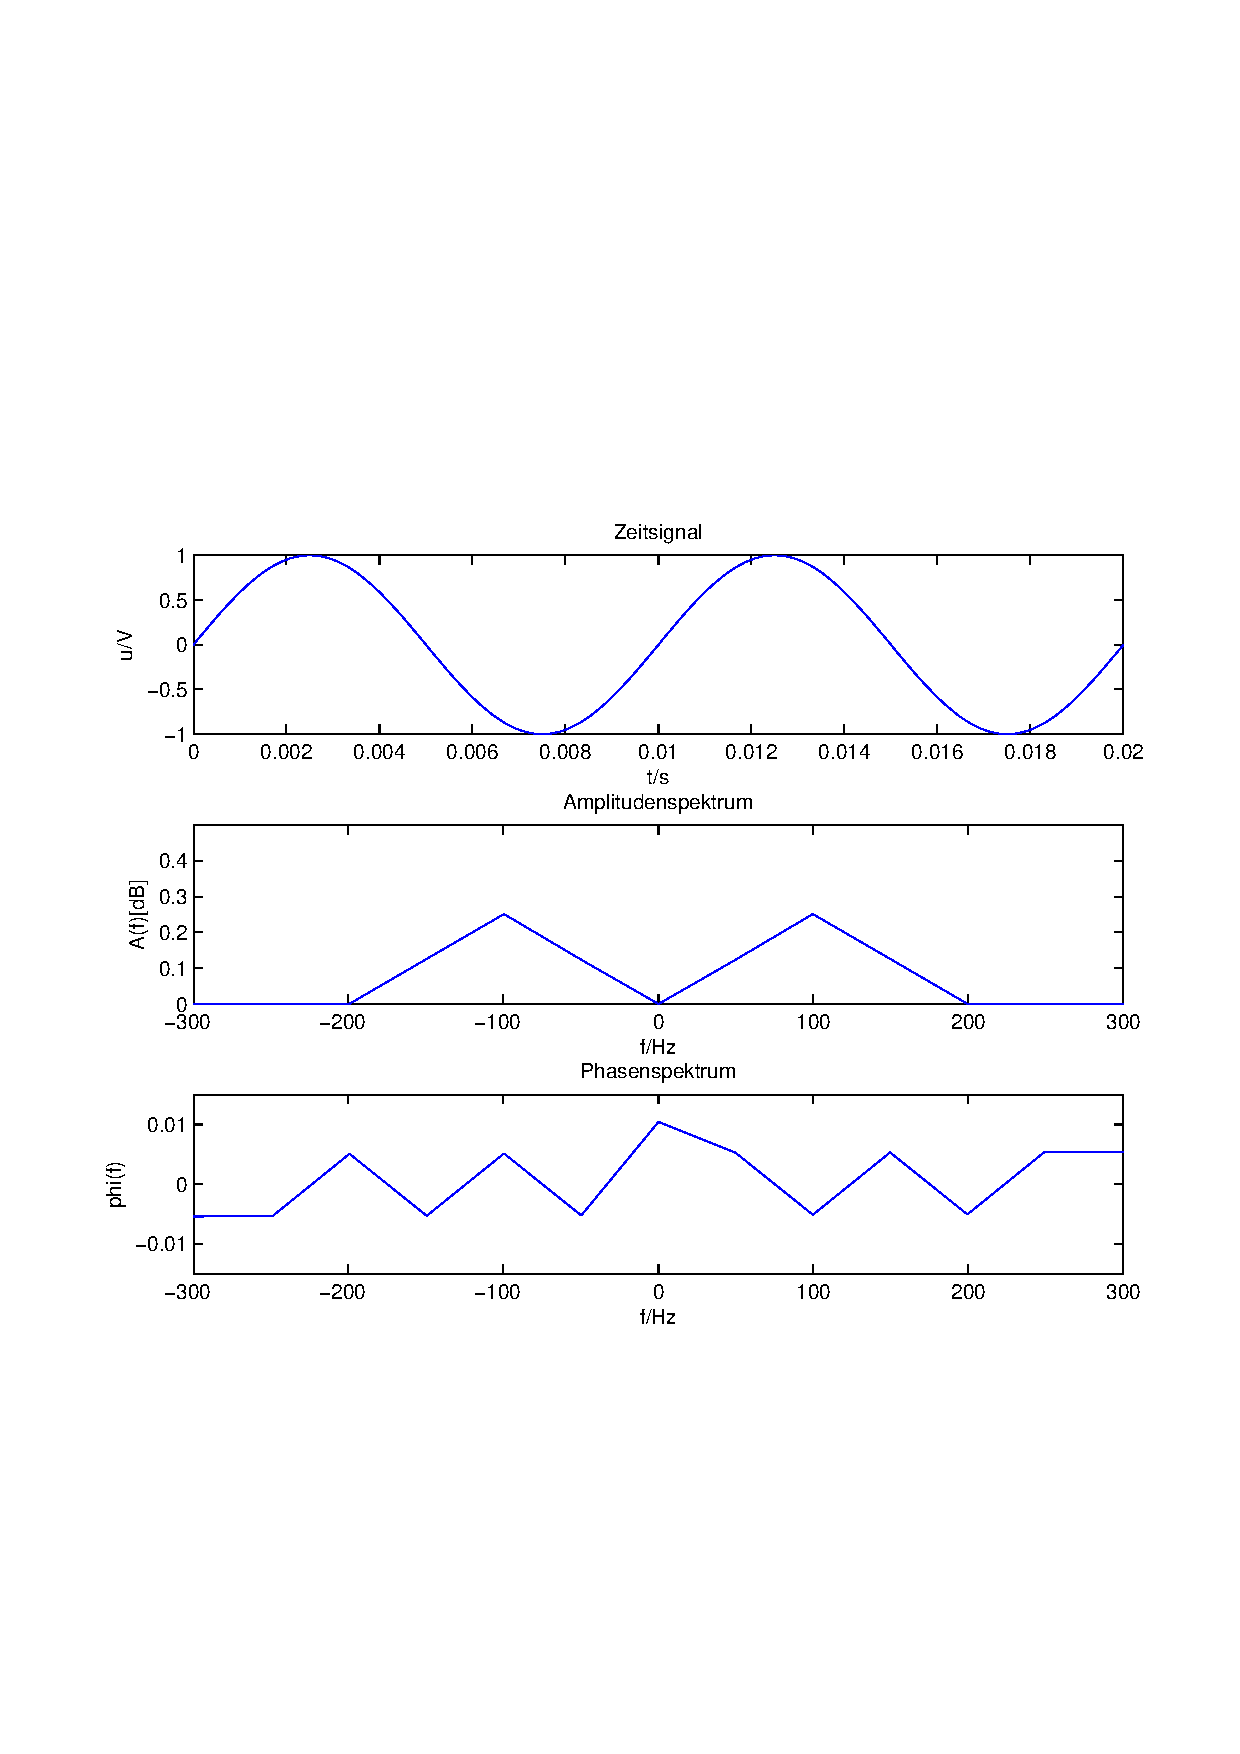
\includegraphics[scale=0.5, trim = 1.5cm 7cm 1.5cm 8cm, clip]{./Bilder/Hanningwindow}
                    \caption{Hanningwindow}
            \end{figure}
            
            \begin{figure}[H]
            \centering
                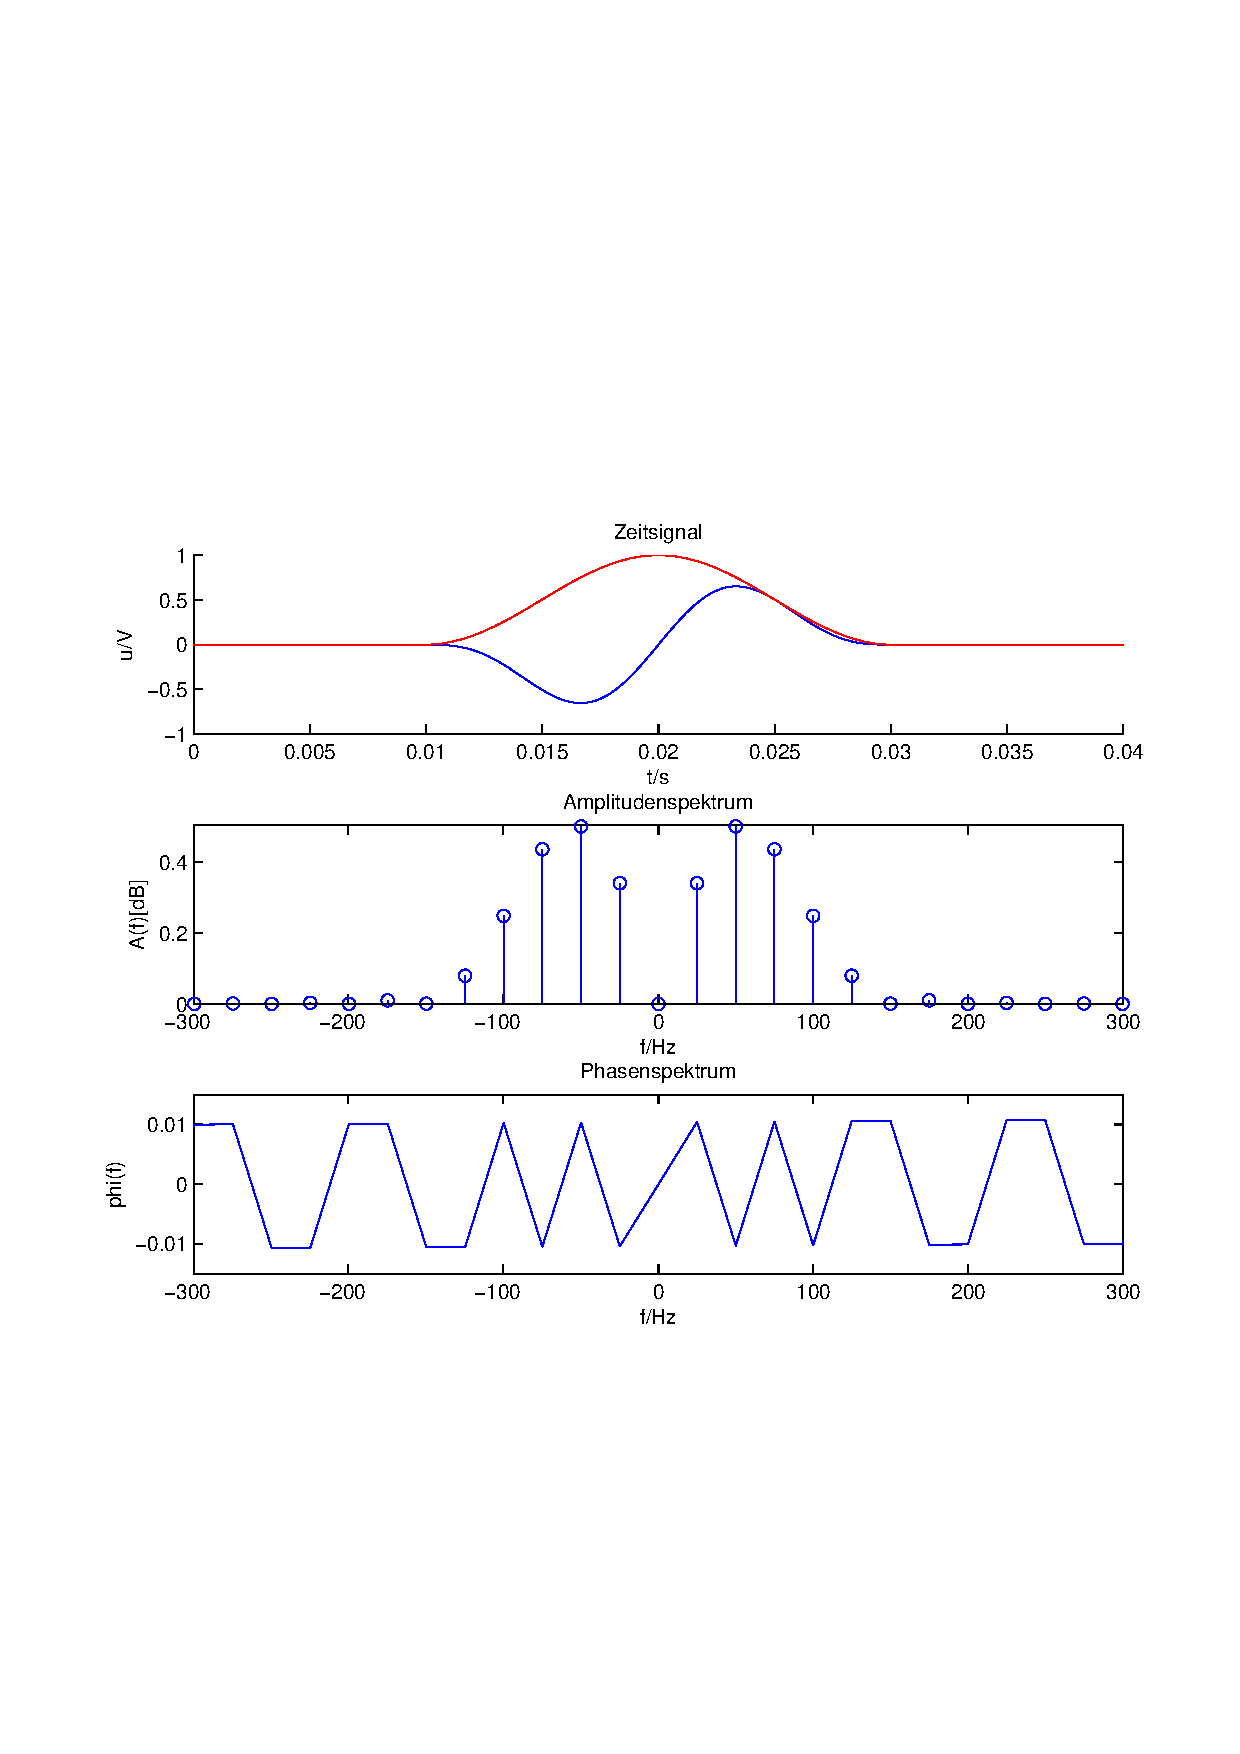
\includegraphics[scale=0.5, trim = 1.5cm 7cm 1.5cm 8cm, clip]{./Bilder/Hanningwindowverkuerzt}
                    \caption{Hanningwindow verkürzt}
            \end{figure}
            
            Die Letzte Simulation zeigt eine Fensterung, die zu dem Leck-Effekt führt. Als Ergebniss ist ein beiteres
            und flacheres Spektrum zu sehen, wie es beim Leckeffekt zu erwarten war.
    			
		\end{quote}

        \subsubsection{DFT eines Rechteck- und Hanningfenster}
		\begin{quote}
            Außerdem untersuchten wir die Spektren von einem Hanning- und einem Rechteckfenster, zuerst mit einer
            Fensterlänge von $16$ und danach mit einer Länge von $2^20$, wobei die restlichen Werte durch Null-Padding
            eingefügt wurden.\\
            Das dazugehörige Skript Vorbereitungsaufgabe43.m befindet sich im Anhang
            Die Plotts dazu sind hier:
            
                %4 Grafiken:
                \begin{center}
                \begin{tabular}{ll}
    
                \hspace{-11em}
                    \begin{minipage}{0.6\textwidth}
    
                        \begin{figure}[H]
                            \label{fig:}
                            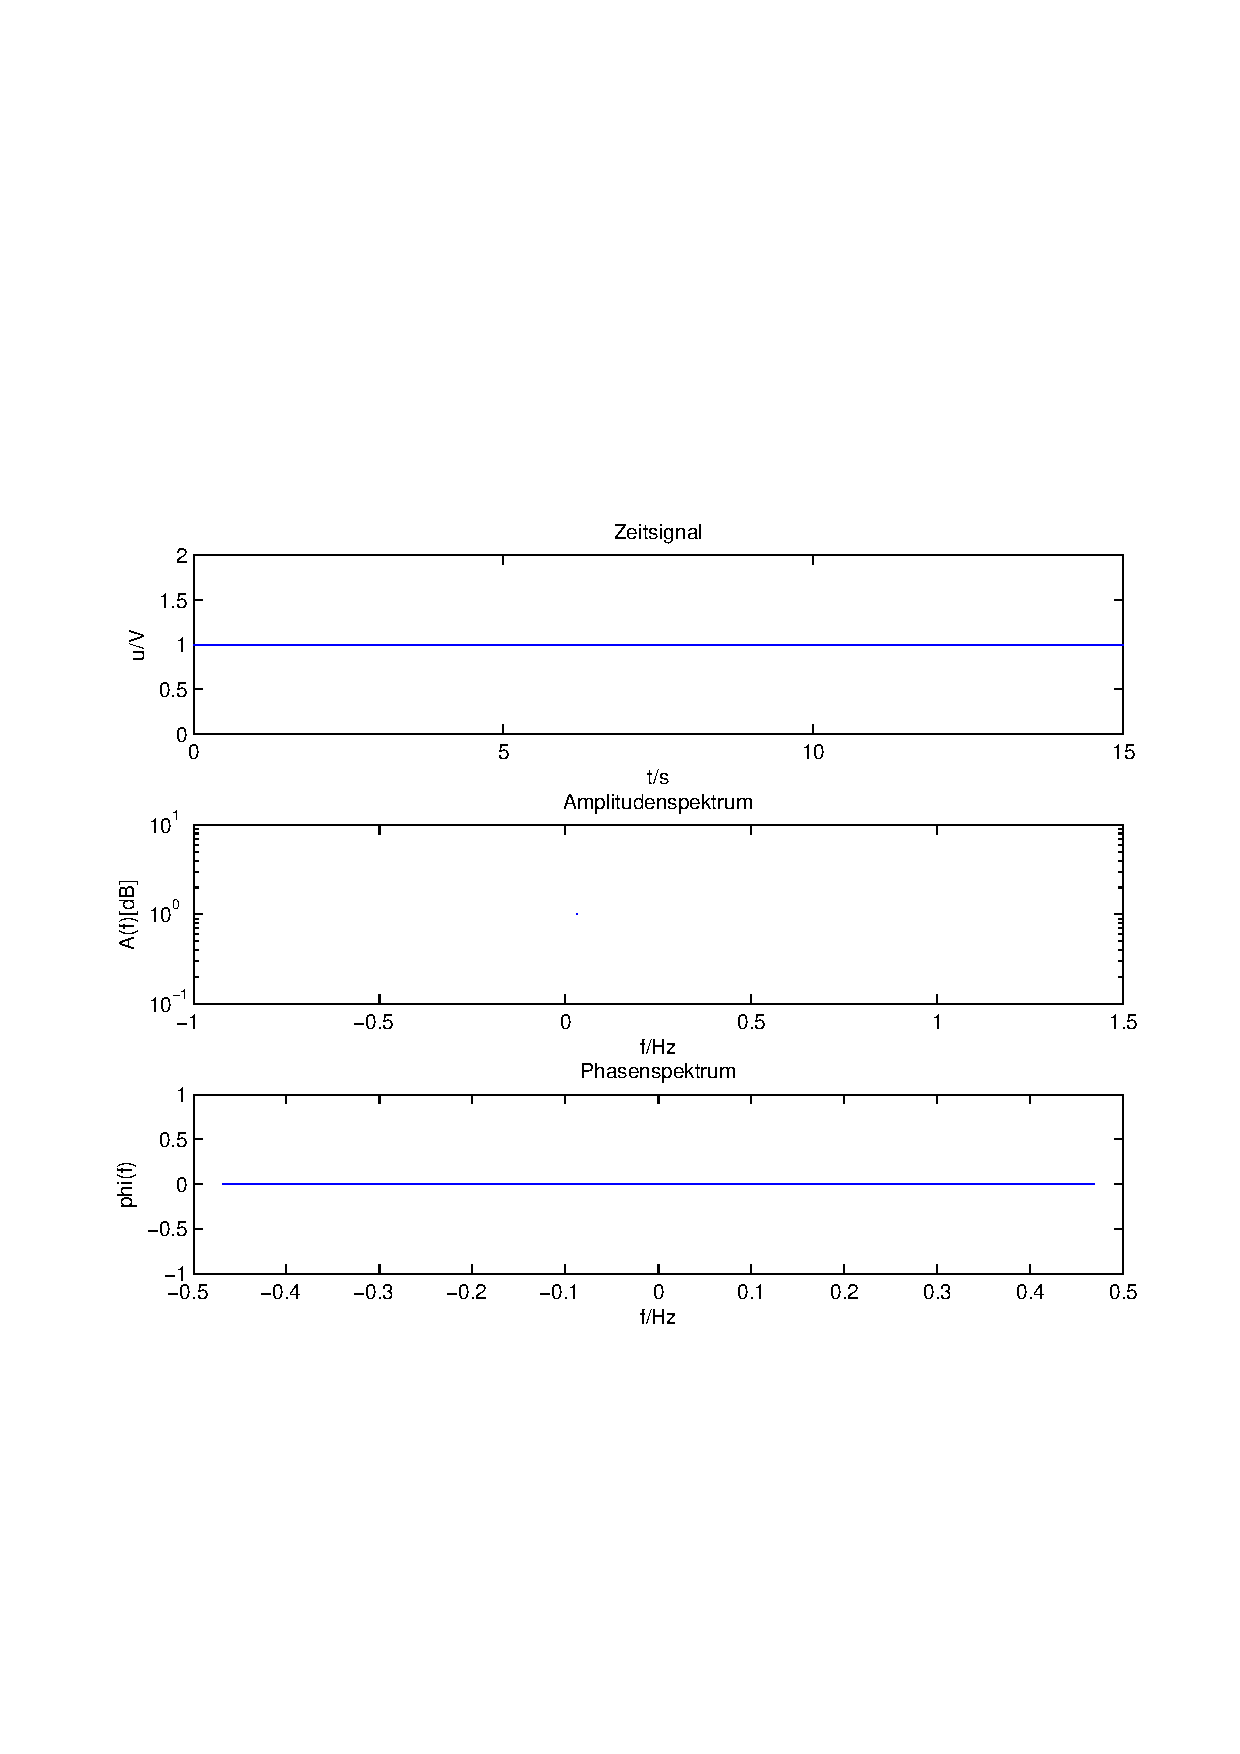
\includegraphics[scale=0.5, trim = 1.5cm 7cm 1.5cm 8cm, clip]{./Bilder/RechteckDFT}
                            %FIXME [width=640px,
                             %height=474px]
                            \caption{DFT eines Rechteckfensters}
                        \end{figure}
    
                    \end{minipage}
                    \begin{minipage}{0.6\textwidth}
    
                        \begin{figure}[H]
                            \label{fig:}
                            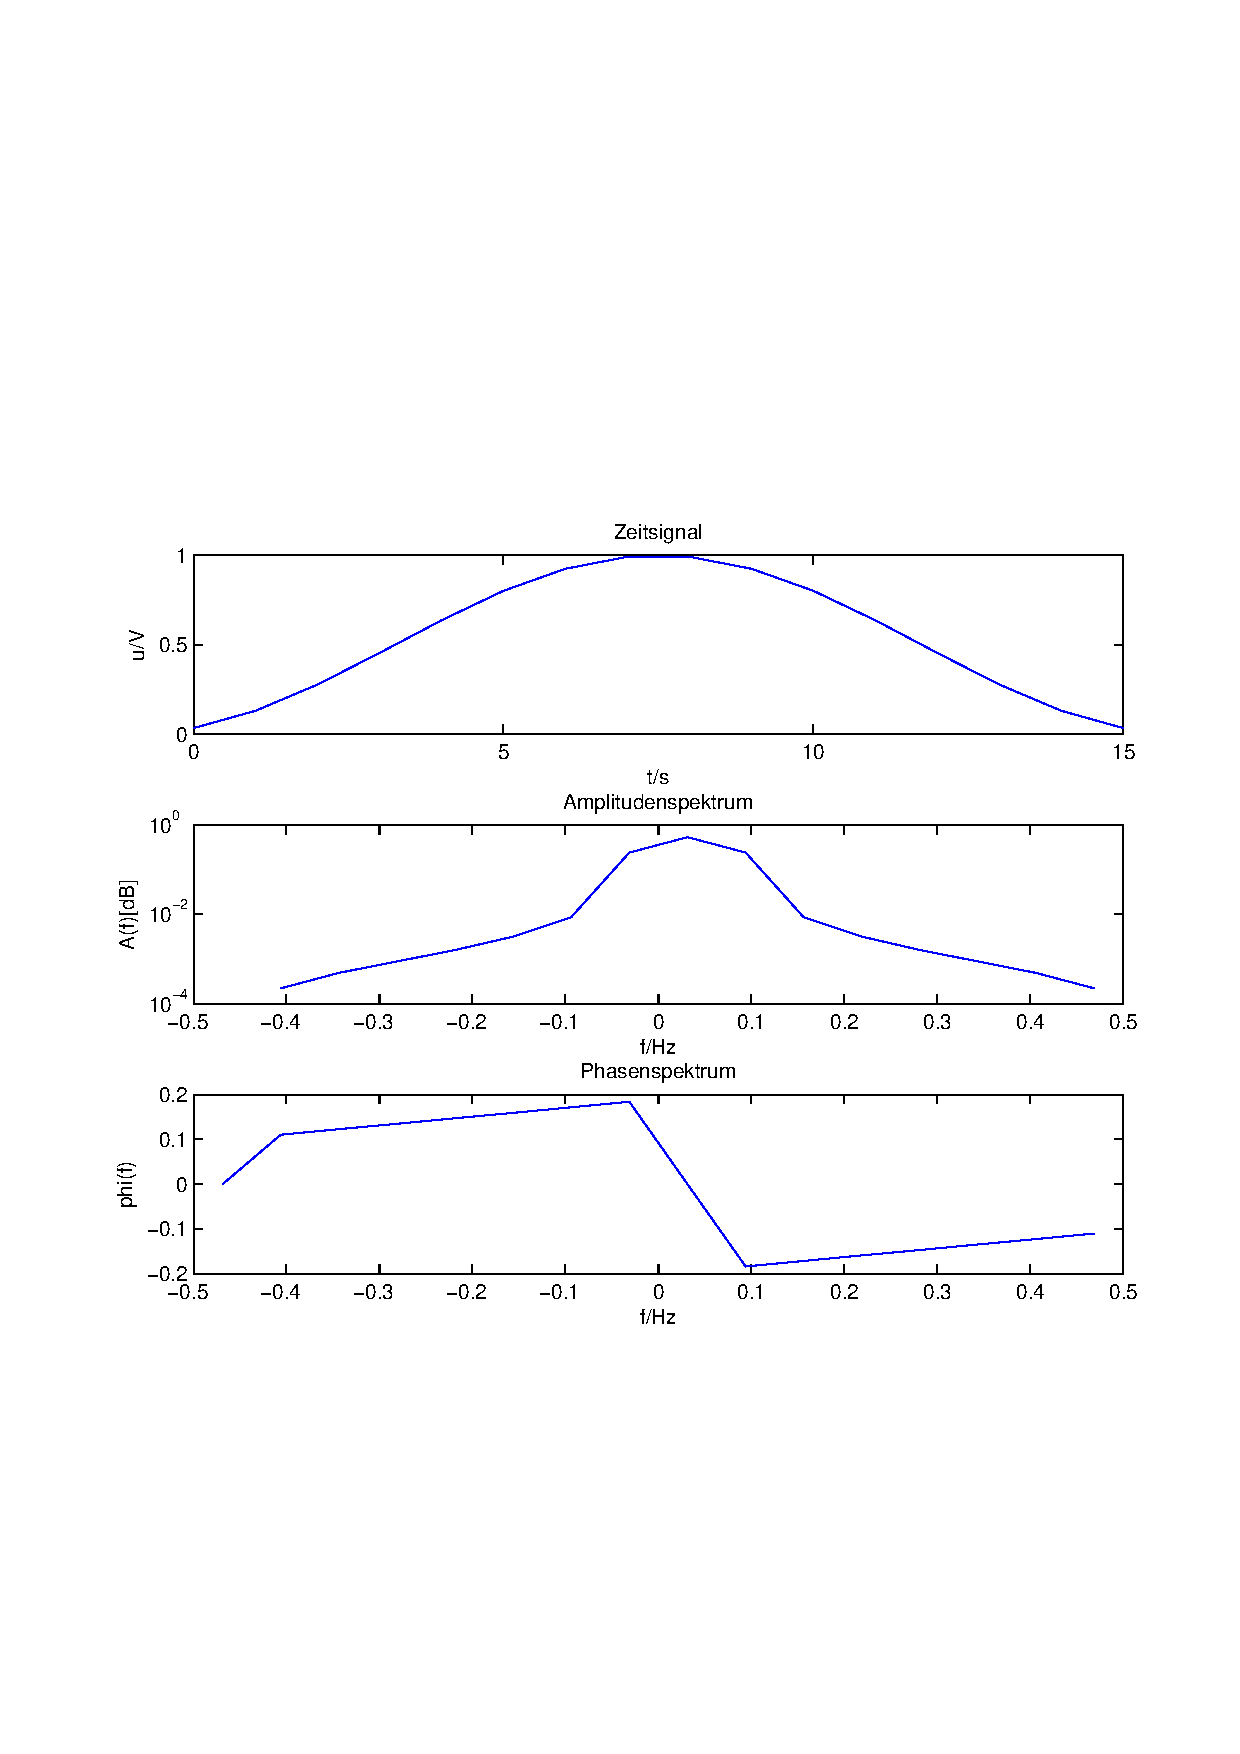
\includegraphics[scale=0.5, trim = 1.5cm 7cm 1.5cm 8cm, clip]{./Bilder/HanningDFT}
                            %FIXME [width=640px,
                             %height=474px]
                            \caption{DFT eines Hanningfensters}
                        \end{figure}
                    \vspace{-1.5em}
    
                    \end{minipage}
    
                \end{tabular}
                \end{center}
    
                            %4 Grafiken:
                \begin{center}
                \begin{tabular}{ll}
    
                \hspace{-11em}
                    \begin{minipage}{0.6\textwidth}
    
                        \begin{figure}[H]
                            \label{fig:}
                            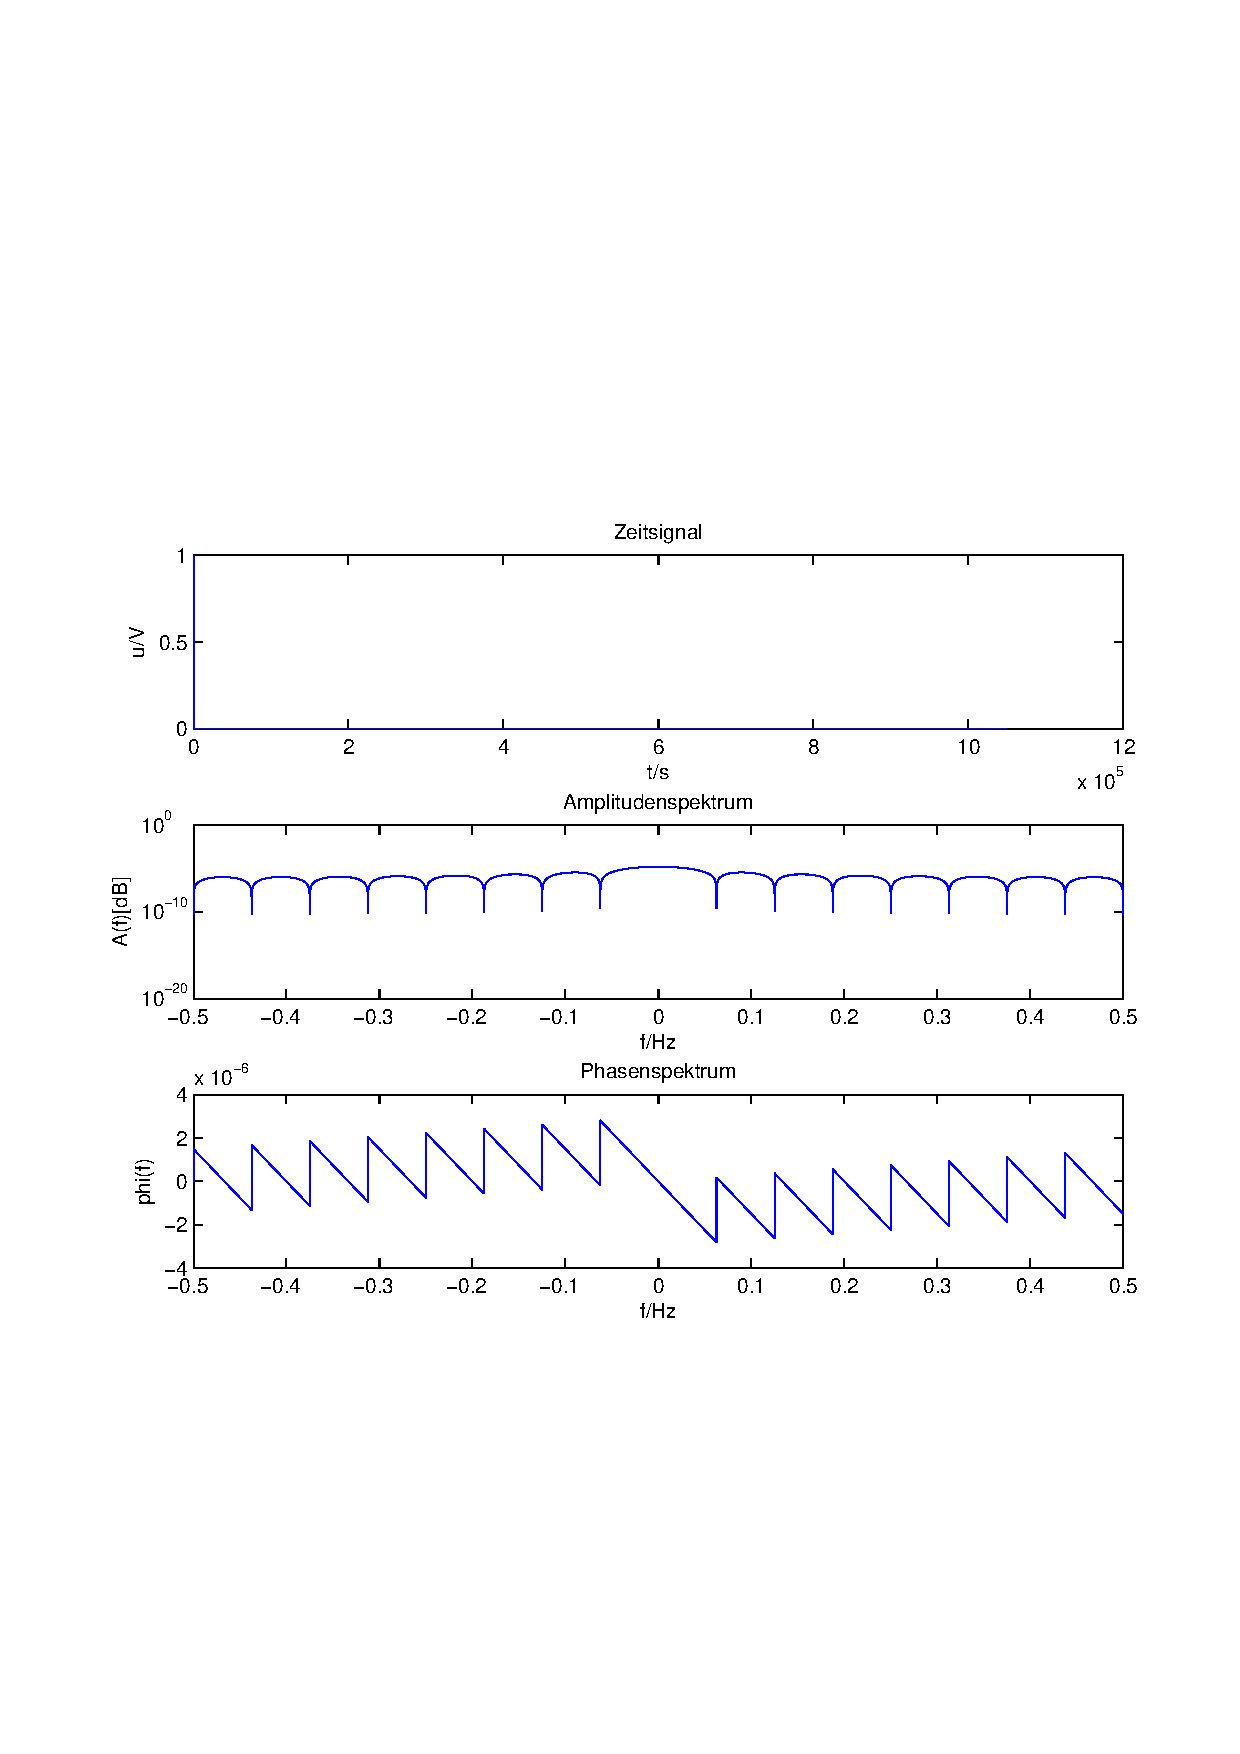
\includegraphics[scale=0.5, trim = 1.5cm 7cm 1.5cm 8cm, clip]{./Bilder/RechteckDFTzeropadding} %FIXME [width=640px,
                            % height=474px]
                            \caption{DFT eines Rechteckfensters mit Zeropadding}
                        \end{figure}
    
                    \end{minipage}
                    \begin{minipage}{0.6\textwidth}
    
                         \begin{figure}[H]
                            \label{fig:}
                            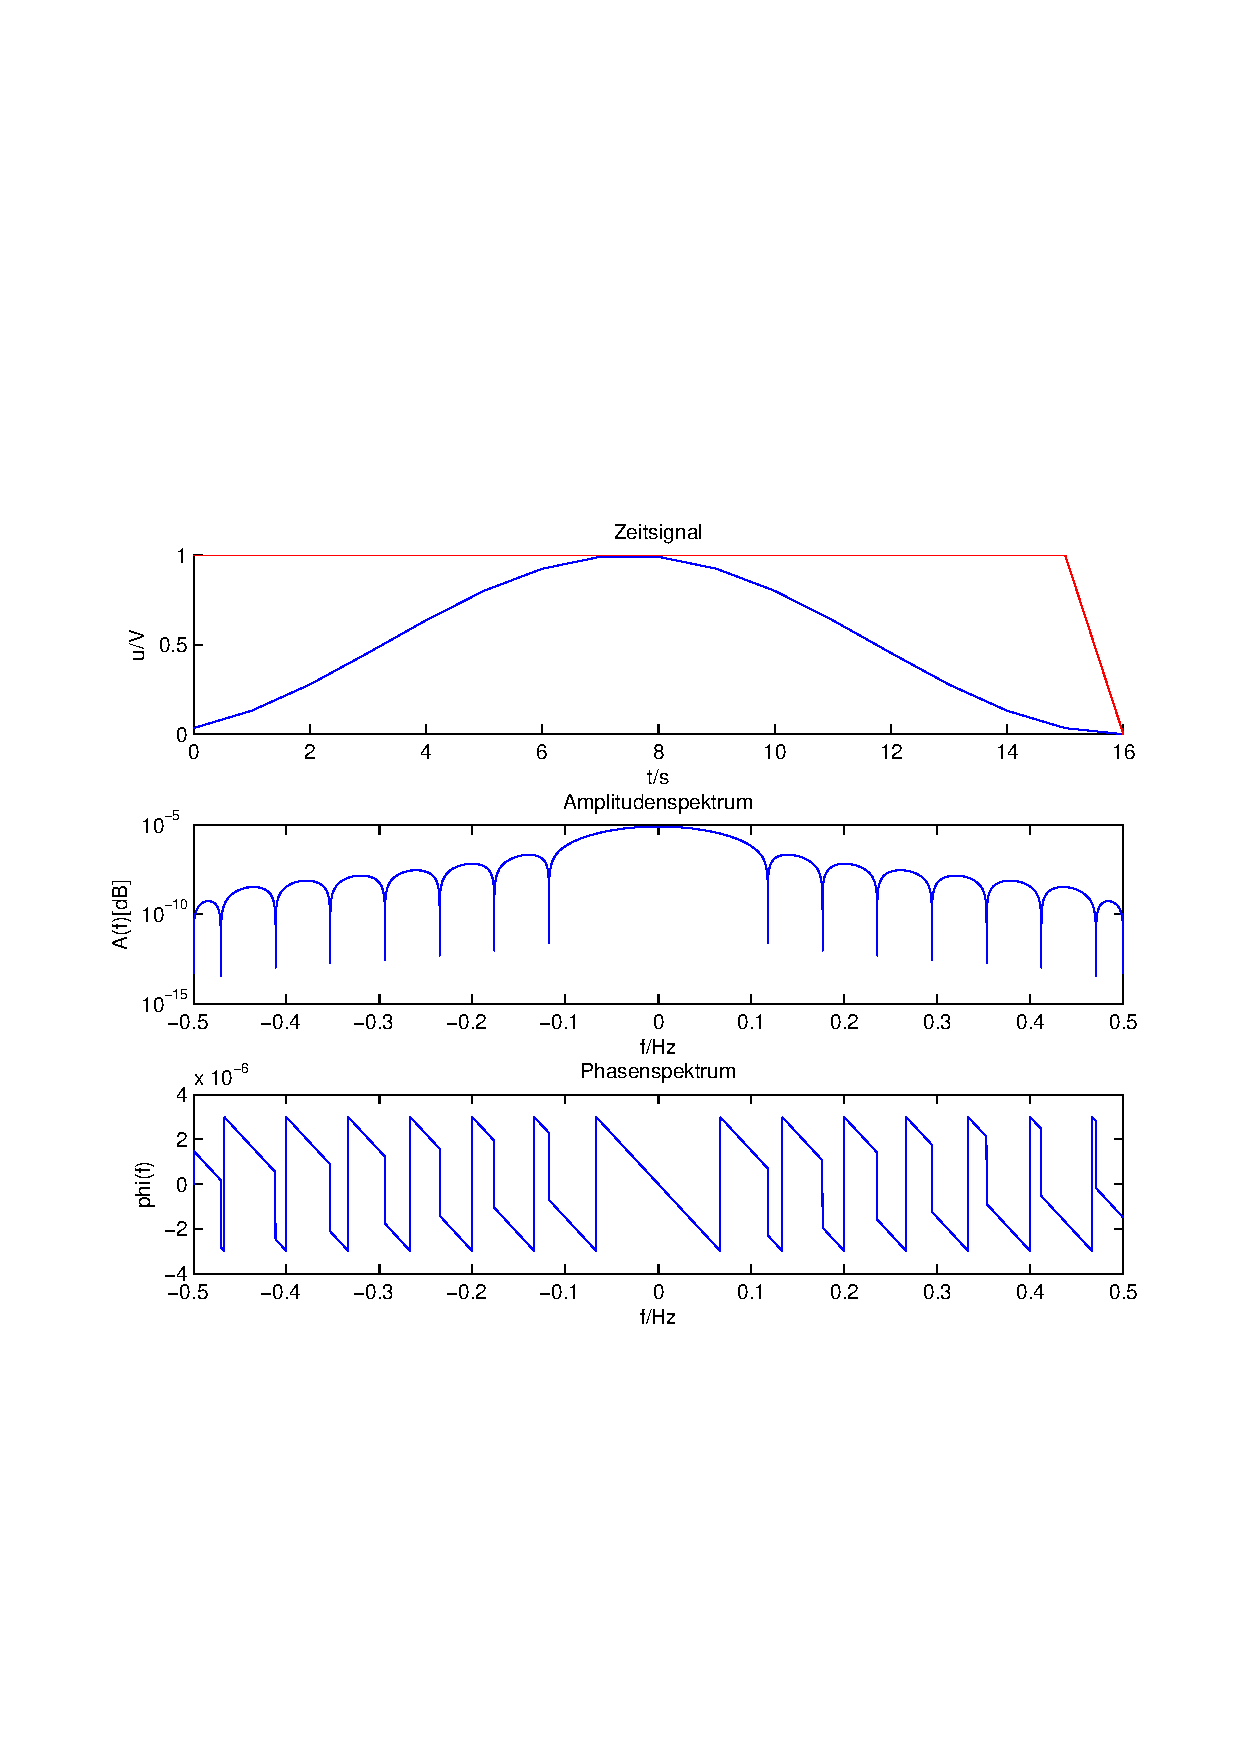
\includegraphics[scale=0.5, trim = 1.5cm 7cm 1.5cm 8cm, clip]{./Bilder/HanningDFTzeropadding} %FIXME [width=640px,
                            % height=474px]
                            \caption{DFT eines Hanningfensters mit Zeropadding}
                        \end{figure}
                   \vspace{-1.5em}
    
                    \end{minipage}
    
                \end{tabular}
                \end{center}
                
            
		\end{quote}
        
        
        
        
        
    \end{quote}
\end{quote}

%--------------------------------------------------------------------
%--------------------------------------------------------------------

\section{Versuch}
\begin{quote}

	\subsection{Schaltungsaufbau}
	\begin{quote}
	Im praktischen Teil des Termins wurden nun reelle Messwerte aufgenommen und
	anhand der Diskreten Fouriertransformation untersucht.\\
	Dazu wurde zunächst eine Schaltung aufgebaut, in der der Strom im
	Dimmerschaltkreis erfasst werden konnte. Der Strom aus der Steckdose führt
	dabei in die Dimmerschaltung und dann in den Stromwandler der Wandler-Box. Dort
	wird das Signal in eine Spannung umgewandelt. Das Verhältnis von Strom zu
	Spannung ist bei dem Wandler linear. Bei einem Maximalstrom von $0.9 A$ kann
	man eine Maximalspannung von $\pm 10 V$ erhalten. Daher muss der Vorfaktor von
	$\frac{0.9 A}{10 V} = 0.09 \frac{A}{V}$ berücksichtigt werden. Noch in der
	Wandler-Box wird dieses Signal gefiltert und führt zum Sensorknoten, wo anhand
	der Spannungsmessung Rückschlüsse auf den Strom gemacht werden können.
	
	\begin{figure}[H]
    \centering
        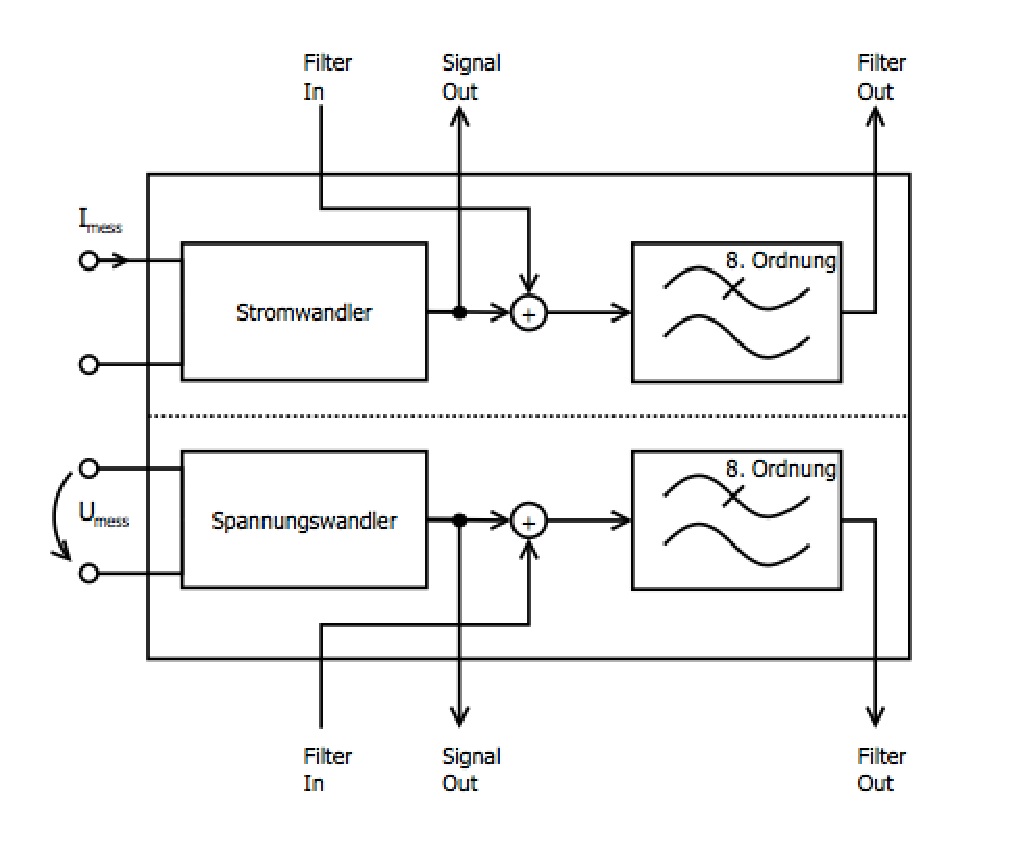
\includegraphics[scale=0.7, trim = 0cm 0cm 0cm 0cm, clip]{./Bilder/Schaltungwandlerbox}
            \caption{Aufbau Wandlerbox}
    \end{figure}
    
	\cite{Schaltungwandlerbox}
	\end{quote}
	
	\subsection{MATLAB-Skript für Anschnittswinkel-Bestimmung}
	\begin{quote}	
	Als nächstes soll anhand eines selbstgeschriebenem MATLAB-Skripts der
	Anschnittswinkel der unterschiedlichen Signale bestimmt werden. Die
	Anschnittswinkel werden dafür vorher mit dem Oszilloskop eingestellt. Da es
	manuell nicht so einfach ist, wurden kleine Abweichungen toleriert.
	
	Unsere anhand des MATLAB-Skripts errechneten Werte wichen nur minimal von den
	erwarteten Anschnittswinkeln ab. Das Ergebnis war also zufriedenstellend. 
    Das dazugehörige Skript ist am Ende des Protokolls zu sehen.
   	\end{quote}
	
	\subsection{Amplituden- und Phasenspektrum des Stroms anhand der Diskreten
	Fouriertransformation}
	\begin{quote}
	\end{quote}
	
	\subsection{Effektivwert des Stroms im Zeit- und Frequenzbereich}
	\begin{quote}
	Zuletzt sollte der Effektivwert des Stroms einer Messung im Zeit- und
	Frequenzbereich ermittelt werden, indem der MATLAB-Skript der
	Vorbereitungsaufgabe verwendet wurde. Wir verwendeten den Strom des Signals bei
	einem Anschnittswinkel von $\frac{\pi}{2}$.\\
	Das MATLAB-Skript gibt uns das Ergebnis von $0.21 A$ für Zeit- und
	Frequenzbereich. Der mithilfe des Multimeters gemessene Strom beträgt $0.224
	A$.\\
	
	Vergleicht man beide Messungen, kann man sehen, dass es keine erhebliche
	Differenz gibt.
	
	 
	\end{quote}
\end{quote}

%--------------------------------------------------------------------
%--------------------------------------------------------------------
\section{Quellcodes}
\begin{quote}
	
	\subsection{Codes aus Termin 3}
	\begin{quote}
	    \subsubsection{sinus2.m}
	    \begin{quote}
	        \lstinputlisting[
	            caption={sinus2},
	            label=lst:Matlab]
	            {./Matlab/sinus2.m}
	    \end{quote}
    
	    \subsubsection{stromPhasSchnitt.m}
	    \begin{quote}
	        \lstinputlisting[
	            caption={stromPhasSchnitt},
	            label=lst:Matlab]
	            {./Matlab/stromPhasSchnitt.m}
	    \end{quote}
    
	    \subsubsection{EffektivwertZeitbereich.m}
	    \begin{quote}
	        \lstinputlisting[
	            caption={EffektivwertZeitbereich},
	            label=lst:Matlab]
	            {./Matlab/EffektivwertZeitbereich.m}
	    \end{quote}
    
	    \subsubsection{EffektivwertFourier.m}
	    \begin{quote}
	        \lstinputlisting[
	            caption={EffektivwertFourier},
	            label=lst:Matlab]
	            {./Matlab/EffektivwertFourier.m}
	    \end{quote}
	    \subsubsection{alphadetektor2.m}
        \begin{quote}
            \lstinputlisting[
                caption={alphadetektor2},
                label=lst:Matlab]
                {./Matlab/alphadetektor2.m}
        \end{quote}
	\end{quote}
	
	\subsection{Codes aus Termin 4}
	\begin{quote}
		
		\subsubsection{Spektrum.m}
		\begin{quote}
		\lstinputlisting[
				caption={Spektrum},
				label=lst:Spektrum]
				{./Matlab/Spektrum.m}
		\end{quote}
		
		\subsubsection{Vorbereitungsaufgabe2.m}
		\begin{quote}
		\lstinputlisting[
				caption={},
				label=lst:Matlab]
		        {./Matlab/Vorbereitungsaufgabe42.m}
		\end{quote}
		
		\subsubsection{Vorbereitungsaufgabe3.m}
		\begin{quote}
		\lstinputlisting[
				caption={Vorbereitungsaufgabe43},
				label=lst:Matlab]
                {./Matlab/Vorbereitungsaufgabe43.m}		
		\end{quote}
		
	\end{quote}
\end{quote}

%--------------------------------------------------------------------
%--------------------------------------------------------------------


\begin{thebibliography}{999}
\bibitem {Schaltungwandlerbox} Prof. Dr.-Ing. Gühmann, Clemens; Dipl.-Ing. Funk, Jürgen: MDVLaborGeraete_web, S.4

%Name, Vorname.; evtl. Name2, Vorname2.: Titel des Dokumentes
%oder Buches, Zeitschrift/Verlag/URL (Auflage, Erscheinungsort, -jahr), ggf. Seitenzahlen
\bibitem {PasevalscheTheorem} \url{https://de.wikipedia.org/wiki/Parsevalsches_Theorem}, Zugriff
23.05.2012
\end{thebibliography}


\end{document}


